\documentclass[conference]{IEEEtran}

\usepackage{graphicx}
\usepackage{amsmath}
\usepackage{amssymb}
\usepackage{booktabs}
\usepackage{multirow}
\usepackage{array}
\usepackage{url}
\usepackage{cite}

\begin{document}

\title{Physics-Guided CBCT-to-Panoramic DRR Synthesis for Dental 2D--3D Data Pairing}

\author{
\IEEEauthorblockN{Aditya Sham Thombare}
\IEEEauthorblockA{Department of Computer Science and Engineering \\
Sardar Vallabhbhai National Institute of Technology \\
Surat, India \\
P24DS005@coed.svnit.ac.in}
\and
\IEEEauthorblockN{Dr. Chandra Prakash}
\IEEEauthorblockA{Department of Computer Science and Engineering \\
Sardar Vallabhbhai National Institute of Technology \\
Surat, India \\
cprakash@coed.svnit.ac.in}
}

\maketitle

\begin{abstract}
Dental panoramic radiography (orthopantomogram, OPG) is the most widely deployed dental imaging modality owing to its low cost and broad clinical availability; however, its inherently two-dimensional nature introduces anatomical overlap and complete loss of depth information. Cone-beam computed tomography (CBCT) overcomes these limitations by providing high-resolution volumetric 3D data, but at substantially higher acquisition cost and radiation burden—factors that limit its use in resource-constrained clinical settings. A critical bottleneck for learning-based 2D-to-3D dental reconstruction research is the scarcity of large-scale, publicly available paired 2D X-ray and 3D CBCT datasets from the same patient.

This paper presents an end-to-end physics-guided pipeline that addresses this data pairing problem by generating synthetic panoramic X-ray images directly from 3D CBCT volumes using a curved-arch digitally reconstructed radiograph (DRR) formulation grounded in Beer--Lambert attenuation physics. The pipeline operates as follows: (1) CBCT volumes are ingested from NIfTI format with full metadata extraction; (2) isotropic resampling, fixed-size volume normalisation to $128^3$ voxels, and Hounsfield-unit-to-attenuation calibration are applied; (3) a \emph{dynamic patient-adaptive parabolic dental arch trajectory} is auto-fitted from a CLAHE-enhanced bone-density projection of the tooth-level Z-band and an anterior-ridge estimate; (4) curved-focal-trough ray tracing is performed with trilinear attenuation sampling and Beer--Lambert line integration along the per-patient trajectory; (5) radiographic post-processing (percentile windowing, gamma correction, unsharp masking) is applied to improve clinical interpretability; and (6) multi-view augmentation and paired dataset packaging are performed for downstream model training.

Applied to 21 CBCT volumes, the pipeline produced 21 base synthetic panoramic DRRs and 63 augmented panoramic variants at rotation offsets of $-3^\circ$, $0^\circ$, and $+3^\circ$. Cross-view quality evaluation on the rot+0deg condition with the dynamic arch reports average L1\,=\,0.02687, SSIM\,=\,0.7467, and PSNR\,=\,29.70\,dB, confirming stable self-consistency of the patient-adaptive projection. The resulting paired CBCT--panoramic dataset, exported as a PyTorch training artifact (187.2\,MB), together with the accompanying visualisation suite, form a practical foundation for future 2D-to-3D dental reconstruction research.
\end{abstract}

\begin{IEEEkeywords}
Dental imaging, CBCT, panoramic X-ray, DRR, Beer-Lambert law, digitally reconstructed radiograph, 2D-to-3D reconstruction, dental arch, focal trough, NIfTI, data augmentation.
\end{IEEEkeywords}

% =========================================================
\section{Introduction}
\label{sec:intro}
% =========================================================

\subsection{Clinical Context and Motivation}

Oral health is intrinsically linked to systemic well-being. Poor dental hygiene is associated with cardiovascular disease, diabetes, and secondary infections, making timely and accurate dental diagnosis an important public health concern. The primary workhorse for dental diagnosis is the panoramic X-ray (OPG/orthopantomogram): a single, wide-field 2D radiograph that captures the full dentition, both jaws, and the temporomandibular joints in one exposure. The effective radiation dose for a modern digital OPG is typically 4--30\,\textmu Sv (roughly 1--3 days of background radiation), and the cost in India ranges from INR\,800--1500.

Despite its widespread use, panoramic radiography collapses a three-dimensional anatomical volume onto a two-dimensional projection plane, causing overlapping structures and complete loss of depth. This limits its utility for tasks requiring spatial assessment, such as implant placement planning, complex molar extractions, root canal morphology evaluation, and detection of subtle inter-radicular bone defects \cite{oliveira2025digital}.

CBCT addresses these limitations by rotating an X-ray source around the patient and reconstructing a full volumetric dataset from hundreds of 2D projections. The resulting 3D volume can be interrogated in axial, coronal, sagittal, and oblique planes, and can be surface-rendered to produce a 3D mesh \cite{oliveira2025digital}. However, CBCT incurs an effective dose of 20--200\,\textmu Sv for small/medium fields of view (up to 530\,\textmu Sv for large FOV or older systems), and costs INR\,1500--6000 in India, placing it out of reach for routine use or for clinics lacking the equipment.

This disparity motivates an alternative strategy: \textit{reconstruct 3D information from widely available 2D panoramic X-rays} \cite{maken20232d}. Recent machine-learning methods have explored this direction \cite{song2021oral,song2023oral,park2024nebla,parida2025vit,ma2024px2tooth,mei2023dtr,li20243dpx,anusree2023deep,wang2024neural}, but all face a shared bottleneck---the lack of large-scale, clinically paired 2D/3D training data from the same patient \cite{sunilkumar2024recent}.

\subsection{Problem Statement}

The development of robust deep learning models for 2D-to-3D dental reconstruction is constrained by:
\begin{itemize}
    \item The scarcity of publicly available, large-scale datasets containing paired 2D panoramic X-rays and 3D CBCT volumes from the same patient.
    \item The assumption of standardized, idealized X-ray acquisition trajectories that may not reflect real-world variation across clinical machines and patients.
    \item The inability of existing approaches to fully capture fine anatomical structures (e.g., root morphology, bone microstructure) critical for clinical planning.
    \item Evaluations that focus on technical image metrics rather than clinically relevant diagnostic outcomes.
\end{itemize}

\subsection{Contributions}

This work directly addresses the data pairing constraint through a physics-guided synthetic data generation pipeline. Specifically, the contributions are:
\begin{itemize}
    \item A complete curved-arch DRR pipeline for CBCT-to-panoramic synthesis with a \emph{dynamic, patient-adaptive parabolic dental arch} that is auto-fitted per volume from a CLAHE-enhanced, morphologically cleaned bone-density projection and an anterior ridge estimate.
    \item A Beer--Lambert projection module with curved-focal-trough ray tracing, trilinear attenuation coefficient sampling, and discrete line integration along the patient-specific trajectory.
    \item Multi-view augmentation at three rotation offsets together with Poisson photon-counting noise and brightness/contrast jitter to improve the diversity of the paired training set.
    \item A paired CBCT--panoramic dataset packaged in PyTorch format, accompanied by quantitative quality verification and rich visualization diagnostics.
\end{itemize}

% =========================================================
\section{Related Work}
\label{sec:related}
% =========================================================

\subsection{2D-to-3D Reconstruction: Surveys and Background}

The general problem of recovering volumetric anatomy from one or a few X-ray projections has been the subject of recent surveys. Maken and Gupta \cite{maken20232d} provide a comprehensive review of computational 3D image reconstruction from X-ray images, motivating the use of X-ray inputs as a low-dose alternative to MRI/CT/CBCT and analysing feature-selection strategies and their applicability across anatomical regions. Oliveira \cite{oliveira2025digital} surveys the broader transition of digital dental radiology from 2D to 3D, discussing how CBCT overcomes 2D limitations such as superimposition and distortion, the role of low-dose protocols and AI-based image analysis, and the place of MRI and ultrasound as non-ionising adjuncts. Sunilkumar \emph{et al.}\ \cite{sunilkumar2024recent} review the methodologies used to synthesise dental panoramic X-rays, focusing on automated synthesis from CBCT/phantoms and the associated clinical advantages and limitations.

\subsection{Neural Radiance Fields for Medical Imaging}

The original NeRF formulation \cite{mildenhall2021nerf} demonstrated that a fully connected multi-layer perceptron (MLP) network can represent a 3D scene as a continuous volumetric radiance field, enabling novel-view synthesis at exceptional quality. Wang \emph{et al.}\ \cite{wang2024neural} present a comprehensive examination of NeRF in medical imaging, highlighting four imminent challenges (fundamental imaging principles, inner-structure requirement, object-boundary definition, and colour--density significance), reviewing methods on different organs and discussing related limitations, datasets and evaluation metrics. NeRF-based reconstruction remains computationally heavy and is sensitive to acquisition assumptions and accurate camera-pose estimation, limiting clinical feasibility.

\subsection{Single-View 2D-to-3D Dental Reconstruction}

\textbf{Oral-3D / Oral-3Dv2.} Oral-3D \cite{song2021oral} introduced a generative-network framework that back-projects a 2D X-ray into 3D space and then registers the generated volume against a prior dental-arch shape, restoring both bony-tissue density and the curved mandible surface from a single panoramic image. Oral-3Dv2 \cite{song2023oral} subsequently re-formulates the problem as learning solely from projection information by mapping 2D coordinates into voxel densities through an implicit neural representation, employing a multi-head model and a dynamic sampling strategy to refine details without paired training images or strong individual priors.

\textbf{X2Teeth and OralViewer.} X2Teeth \cite{liang2020x2teeth} decomposes the multi-tooth reconstruction task into teeth localisation and single-shape estimation, and is trained patch-wise to reconstruct the full cavity from one panoramic radiograph. The same line of work led to OralViewer \cite{liang2021oralviewer}, an interactive system that combines a per-patient 3D-teeth reconstruction model from a single panoramic X-ray with registered gum and jaw-bone meshes, providing 3D demonstration of dental surgeries for patient education.

\textbf{NeBLa and ViT-NeBLa.} NeBLa \cite{park2024nebla} introduces a Beer--Lambert-inspired pipeline that creates an intermediate ``simulated PX'' (SimPX) image from CBCT, then learns a ray-tracing-based neural model that maps SimPX to 3D, while bypassing the need for matched PX/CBCT pairs and dental-arch priors at inference. ViT--NeBLa \cite{parida2025vit} extends this physics-guided design with a hybrid Vision-Transformer/CNN backbone and a learnable multi-resolution hash positional encoding; importantly, projection rays are parameterised by tangency to a \emph{patient-adaptive elliptical path} and sampling is restricted to a jaw-focused horseshoe focal trough, removing the intermediate density-aggregation step and reducing per-ray samples by approximately 52\%.

\textbf{PX2Tooth and DTR-Net.} PX2Tooth \cite{ma2024px2tooth} reconstructs 3D point-cloud teeth from a single panoramic X-ray with a two-stage pipeline (PXSegNet for tooth segmentation and TGNet with a Prior Fusion Module for point-cloud generation), reporting an IoU of 0.793 on a 499-pair CBCT/PX dataset. DTR-Net \cite{mei2023dtr} pursues a complementary dual-space strategy: an image-space 2D-to-3D generative branch (guided by a tooth-segmentation task) is paired with a geometric-space implicit-function branch that uses points to capture complicated tooth shapes, achieving state-of-the-art 3D tooth reconstruction quality.

\textbf{3DPX and Attention U-Net (Anusree).} Li \emph{et al.}\ \cite{li20243dpx} propose 3DPX, a progressive hybrid MLP--CNN pyramid network that imposes intermediate guidance at each pyramid level and combines MLPs with CNNs to capture long-range dependencies during 2D-to-3D oral reconstruction, reporting improved reconstruction and downstream tooth-angular-misalignment classification on two large datasets. The earlier Attention U-Net study by Anusree and You \cite{anusree2023deep} evaluates the suitability of an attention-augmented U-Net for reconstructing flattened CBCT volumes across the dental arch from 2D panoramic X-rays, showing improvements over plain auto-encoders in both quantitative scores and perceptual quality.

\textbf{Multi-View and Application-Specific Reconstruction.} Mohamed \emph{et al.}\ \cite{mohamed20253d} present a 3D reconstruction model from 2D multi-view dental images based on EfficientNetB0 with a 3D-LSTM recurrence stage, reporting an IoU of 89.98\% and an F1-score of 94.11\% on ShapeNet and a custom dental dataset. Minhas \emph{et al.}\ \cite{minhas2024artificial} explore a generative deep-learning algorithm for reconstructing pseudo-3D representations of maxillary impacted canines from 2D panoramic X-rays, reporting an SSIM of 0.71 and case-level positional-prediction accuracy in the buccolingual and mesiodistal directions.

\textbf{Bone Surface and Benchmark Studies.} Beyond the dental cavity, Gu \emph{et al.}\ \cite{gu20243ddx} propose 3DDX, a method that learns multiple front- and back-surface depth maps from a single standard-geometry radiograph and exploits the fixed X-ray geometry to reduce surface reconstruction error from 4.78\,mm to 1.96\,mm on hip CT/X-ray data. Shakya and Khanal \cite{shakya2023benchmarking} benchmark eight encoder--decoder architectures for biplanar X-ray to 3D bone-shape reconstruction across six public datasets, observing that attention-based methods generalise best across anatomies and that segmentation-style metrics can over-estimate clinical-parameter accuracy.

\subsection{CBCT-to-Panoramic Synthesis}

The closest line of work to ours is the synthesis of panoramic images directly from CBCT. Sunilkumar \emph{et al.}\ \cite{sunilkumar2025panoramic} propose a robust simulated-geometry method that adjusts the ray trajectory to be optimal for a patient's jaw shape, achieves uniform ray sampling by progressively increasing sampling intervals, and applies tilt correction to compensate for incorrect patient positioning, outperforming both prior simulated-geometry approaches and image-processing baselines. Their patient-tailored, scan-parameter-free formulation directly motivates the curved-arch and patient-adaptive trajectory design adopted in this work.

\subsection{Sparse-View and Reconstruction-Based CBCT}

A complementary body of work targets CBCT reconstruction itself from very few X-ray projections, which conceptually inverts the synthesis problem we address. DIF-Net \cite{lin2023learning} formulates the CT volume as a continuous intensity field and regresses per-point intensities from a small number of view-specific 2D features, enabling reconstruction from extremely sparse views in $\sim$1.6\,s. C\textsuperscript{2}RV \cite{lin2024c} extends this with explicit multi-scale volumetric representations and a scale-view cross-attention module, reporting consistent improvements across diverse anatomies. Liu \emph{et al.}\ \cite{liu2024geometry} introduce a geometry-aware encoder--decoder that back-projects multi-view 2D features into 3D space along the CBCT scanning geometry, supporting extremely sparse inputs (5--10 views) without per-scan optimisation. DeepSparse \cite{lin2026deepsparse} pushes this further as a foundation model with a Dual-Dimensional Cross-Scale Embedding (DiCE) backbone and a HyViP pretraining/finetuning framework. Trans\textsuperscript{2}-CBCT \cite{yang2025trans} couples a TransUNet hybrid CNN--Transformer feature extractor with a neighbour-aware Point Transformer to enforce volumetric coherence, reporting improvements on LUNA16 and ToothFairy. DiffVox \cite{momeni2024differentiable} demonstrates that exact discrete Beer--Lambert rendering inside a differentiable voxel-based optimiser outperforms iterative reconstruction algorithms and modern neural fields, particularly under few-view conditions, validating the choice of an explicit Beer--Lambert formulation. Zhang \emph{et al.}\ \cite{zhang2023novel} propose a 3D sparse-view CBCT reconstruction algorithm that combines weighted Schatten p-norm minimisation (WSNM) with a TV-regularised ASD-POCS update, improving RMSE, PSNR, and SSIM on phantom and clinical data. Shin \emph{et al.}\ \cite{shin2025sparse} address the same problem with a meta-learned neural attenuation field regularised by hash-encoding, again confirming the value of physics-guided neural methods for dose reduction.

\subsection{Dynamic and Time-Resolved CBCT}

For applications where intra-scan motion matters, Xie \emph{et al.}\ \cite{xie2025time} propose PMF-STGR, a prior-model-free spatiotemporal Gaussian-representation framework that reconstructs a sequence of CBCTs (one per X-ray projection) from a standard 3D scan in a one-shot training fashion, reporting reduced reconstruction time and improved motion accuracy compared with implicit-neural-representation-based PMF-STINR.

\subsection{Mandible Segmentation and Intraoral Surface Labelling}

Although our work focuses on synthesis rather than segmentation, two related contributions inform our arch geometry assumptions. Abdi \emph{et al.}\ \cite{abdi2015automatic} develop an atlas-assisted mandible segmentation method for panoramic X-rays based on horizontal integral projections, modified Canny edges and contour tracing, achieving $>$93\% Dice/specificity/sensitivity on 95 panoramic X-rays. Lian \emph{et al.}\ \cite{lian2020deep} introduce MeshSegNet, an end-to-end multi-scale mesh-feature learning method for tooth labelling on raw 3D intraoral scanner surfaces, capturing fine-grained local geometric context that pure point-cloud methods miss. These works confirm that anatomically-aware geometric priors substantially improve dental shape understanding---an observation that supports our choice of an auto-fitted parabolic arch in the projection model.

\subsection{Positioning of This Work}

The above methods collectively rely on paired or at minimum semi-paired 2D/3D data for training and evaluation \cite{park2024nebla,parida2025vit,ma2024px2tooth,song2023oral}. Our work occupies a complementary position: rather than performing reconstruction, we focus on \textit{generating} paired training data from available CBCT volumes using explicit Beer--Lambert projection physics and a curved, patient-adaptive dental trajectory model in the spirit of the patient-tailored simulated geometry of \cite{sunilkumar2025panoramic}. The synthetic panoramics produced serve as input for downstream reconstruction models such as those above.

% =========================================================
\section{Domain Background: Dental Anatomy and Imaging Physics}
\label{sec:background}
% =========================================================

\subsection{Dental Anatomy}

The human dentition consists of incisors, canines, premolars, and molars arranged in the upper (maxillary) and lower (mandibular) jaws. Key anatomical structures relevant to imaging include: the enamel (hardest tissue in the body, high X-ray attenuation), dentin (supporting layer beneath enamel, moderate attenuation), the pulp chamber (soft tissue, low attenuation), cementum, the periodontal ligament anchoring the tooth root, and the alveolar bone forming the tooth sockets.

Dental diseases include caries (bacterial breakdown of enamel progressing through dentin to pulp), gingivitis and periodontitis (gum inflammation leading to bone loss), tooth sensitivity from exposed dentin, and malocclusion from crowding or bite misalignment. Accurate imaging of these structures motivates the use of CBCT for planning implants, complex extractions, root canal evaluation, and jaw pathology analysis.

\subsection{Dental Imaging Modalities}

Table~\ref{tab:modalities} summarizes the four primary radiographic modalities used in dentistry. Panoramic radiography provides the broadest field of view but is limited to 2D projection. CBCT provides full 3D volumetric data—viewable in axial, coronal, sagittal, and 3D-mesh representations—at the cost of higher dose and equipment expense.

\begin{table}[t]
\caption{Comparison of Dental Radiographic Modalities}
\label{tab:modalities}
\centering
\setlength{\tabcolsep}{3pt}
\begin{tabular}{p{1.55cm} p{1.7cm} p{2.55cm} p{0.6cm}}
\toprule
\textbf{Modality} & \textbf{Effective Dose} & \textbf{Key Use} & \textbf{Dim.} \\
\midrule
Intraoral (PA/BWX) & 1.5--8.2\,\textmu Sv & Caries, root, bone level & 2D \\
Panoramic (OPG)   & 4--30\,\textmu Sv   & Impaction, cysts, tumours & 2D \\
CBCT (small/med FOV) & 20--200\,\textmu Sv & Implants, canals, fractures & 3D \\
CBCT (large FOV)  & Up to 530\,\textmu Sv & Full jaw pathology & 3D \\
\bottomrule
\end{tabular}
\end{table}

\subsection{Digitally Reconstructed Radiograph (DRR)}

A DRR is a synthetic 2D X-ray generated by computationally projecting a 3D volumetric dataset (such as CBCT) along a defined ray geometry, integrating the linear attenuation coefficient $\mu(\mathbf{x})$ along each ray according to the Beer-Lambert law. DRRs are commonly used for imaging simulation, multi-modal registration, and—as in this work—generating training data by creating synthetic panoramic images from CBCT volumes.

\subsection{Beer-Lambert Law}

The fundamental physical model governing X-ray attenuation through tissue is the Beer-Lambert law:
\begin{equation}
I = I_0 \exp\!\left(-\int_{\mathcal{L}} \mu(\mathbf{x})\,d\ell\right),
\label{eq:beer}
\end{equation}
where $I_0$ is the incident beam intensity, $I$ is the transmitted intensity, $\mu(\mathbf{x})$ is the linear attenuation coefficient at spatial position $\mathbf{x}$, and the integral is taken along ray path $\mathcal{L}$. Tissue attenuation values in mm$^{-1}$ are approximately: air $\approx$0 (suppressed), soft tissue $\approx$0.01--0.025, bone $\approx$0.025--0.08, and dense enamel/metal $\approx$0.08 (clamped upper bound). These values imply that a 30\,mm focal-trough path through bone ($\mu=0.05$) yields an integral of 1.5, corresponding to a transmitted intensity of $\exp(-1.5)\approx0.22$—providing good radiographic contrast between bone and soft tissue.

% =========================================================
\section{Dataset and Preprocessing}
\label{sec:data}
% =========================================================

\subsection{CBCT Dataset}

The current implementation processes 21 CBCT volumes stored in NIfTI (\texttt{.nii}) format, loaded from the project asset directory. All volumes share a consistent acquisition geometry: shape $(604, 604, 412)$ voxels with isotropic in-plane spacing of approximately $0.249\times0.249$\,mm and axial spacing of $0.25$\,mm. Intensity ranges vary across subjects (e.g., $[-2628, 5509]$ to $[-4904, 11129]$ HU), reflecting natural inter-subject variation in bone density and the presence of metallic restorations. Metadata extracted per volume includes: filename, voxel shape, voxel spacing (from header \texttt{get\_zooms()}), affine transform matrix, and intensity statistics (min, max, mean).

\subsection{Preprocessing Pipeline}

Each volume undergoes a three-stage preprocessing pipeline (Fig.~\ref{fig:full_pipeline}):

\textbf{Stage 1 — Isotropic Resampling.} Volumes are resampled to isotropic voxel spacing (1.0\,mm) using SciPy zoom with first-order (trilinear) interpolation. Resampling factors are computed per axis as $f_i = s_i / t_i$, where $s_i$ is the original spacing and $t_i=1.0$\,mm is the target spacing.

\textbf{Stage 2 — Fixed-Size Normalization.} The isotropically resampled volume is further resized to a fixed cubic grid of $128^3$ voxels using PyTorch \texttt{F.interpolate} with trilinear mode. This standardization ensures consistent tensor dimensions across all volumes for batched training.

\textbf{Stage 3 — Attenuation Calibration.} Raw Hounsfield-like intensity values are converted to linear attenuation coefficients $\mu$ (mm$^{-1}$) for physically meaningful Beer-Lambert projection. The piecewise mapping is:
\begin{itemize}
    \item $\text{HU} < -200$: air, $\mu = 0$ (suppressed);
    \item $-200 \leq \text{HU} < 300$: soft tissue window, $\mu = 0.01 + \frac{(\text{HU}+200)}{500} \times 0.015$;
    \item $300 \leq \text{HU} < 3000$: bone window, $\mu = 0.025 + \frac{(\text{HU}-300)}{2700} \times 0.055$;
    \item $\text{HU} \geq 3000$: dense bone/enamel/metal, $\mu$ clamped at 0.08.
\end{itemize}
After preprocessing, all volumes exhibit $\mu \in [0.00000, 0.08000]$, with air fractions of 40.8--49.8\% and bone fractions of 8.5--16.1\% across the 21 subjects. Volumes are converted to PyTorch tensors for downstream processing.

% =========================================================
\section{Methodology}
\label{sec:method}
% =========================================================

\begin{figure*}[t]
\centering
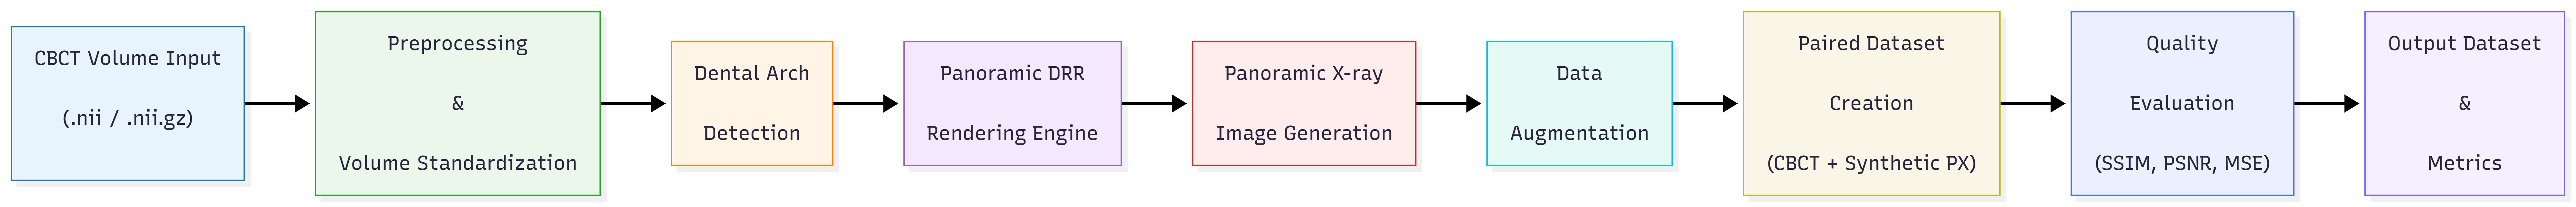
\includegraphics[width=0.92\textwidth]{CBCT Volume Processing.png}
\caption{End-to-end CBCT-to-panoramic DRR pipeline architecture. The pipeline flows from NIfTI ingestion and metadata storage through preprocessing (isotropic resampling, volume normalization, HU-to-attenuation conversion), dental arch detection and geometry modeling, panoramic DRR rendering (curved-focal-trough trilinear sampling), augmentation, paired dataset packaging, and quality metric evaluation via DataLoader.}
\label{fig:full_pipeline}
\end{figure*}

\subsection{Dynamic Patient-Adaptive Dental Arch Geometry}

A key distinguishing feature of panoramic radiography---compared with conventional planar DRR---is that the X-ray source does not traverse a straight line. Instead, the imaging system follows a curved trajectory that traces the dental arch, ensuring that the teeth are optimally in focus throughout the panoramic sweep. Replicating this behaviour requires estimating a patient-specific dental arch curve from each CBCT volume rather than relying on a hard-coded canonical arch. This requirement is consistent with the patient-tailored simulated geometry advocated in \cite{sunilkumar2025panoramic} and the patient-adaptive elliptical projection path used in \cite{parida2025vit}.

To this end, the pipeline implements a \emph{dynamic parabolic arch detector} that automatically estimates the four arch parameters $(c_x, c_y, w, d)$---horizontal centre, anterior--posterior centre, half-width and depth---directly from the bone distribution of each preprocessed CBCT volume. The detector operates on axial bone-density projections of the dental Z-band and consists of the three filtering steps below (Fig.~\ref{fig:arch_geom}).

\textbf{FIX1 -- Tooth-level Z-band restriction.} Analysis is restricted to the axial slabs at $55\%$--$70\%$ of the volume's z-extent, which empirically isolates the tooth-bearing region while excluding the skull base and the upper maxilla. Bone voxels in this band are counted column-wise to form a 2D bone-density projection $B(x,y) = \sum_{z\in\text{Z-band}} \mathbf{1}[\mu(x,y,z)>0.025]$.

\textbf{Pre-processing.} The bone-density projection is normalised to $[0,1]$, contrast-enhanced with Contrast-Limited Adaptive Histogram Equalisation (CLAHE, clip-limit $0.03$, $256$ bins), and smoothed by a Gaussian filter ($\sigma = 1.5$). Otsu thresholding (with a small additive margin) yields a candidate bone mask, which is then cleaned by removal of small objects ($<30$\,px), binary closing with a disk-of-radius-4 structuring element, and small-hole filling ($<300$\,px).

\textbf{FIX2 -- Anterior--posterior band.} Only the $40\%$--$80\%$ AP band is retained, suppressing posterior skull-base bone that would otherwise pull the centroid backward.

\textbf{FIX3 -- Largest connected component.} Connected-component labelling is applied and only the largest component is kept, eliminating spurious fragments coming from metallic restorations or noise. If the surviving mask contains fewer than 50 voxels, the detector reports failure and the pipeline falls back to a hard-coded canonical arch.

From the surviving mask, the arch parameters are derived from the bone footprint:
\begin{align}
    c_x &= \overline{x_{\text{bone}}},\quad c_y = \overline{y_{\text{bone}}}, \nonumber\\
    L_{\text{LR}} &= \max(x_{\text{bone}}) - \min(x_{\text{bone}}), \nonumber\\
    L_{\text{AP}} &= \max(y_{\text{bone}}) - \min(y_{\text{bone}}), \nonumber\\
    w &= 0.42\,L_{\text{LR}},\quad d = 0.20\,L_{\text{AP}}.
    \label{eq:arch}
\end{align}
A column-wise scan of the bone mask additionally extracts an \emph{anterior ridge} $\{(x_i, y_i^{+})\}$, where $y_i^{+}$ is the highest AP coordinate occupied by bone in column $x_i$. The 90$^{\text{th}}$ percentile of the central third of $\{y_i^{+}\}$ provides a robust estimate $y_{\text{ant}}$ of the true anterior arch boundary; $c_y$ is then offset toward this anterior ridge so that the arch vertex (incisors) sits near the actual anterior bone edge.

The final parabolic arch curve is generated in the axial plane as
\begin{equation}
    \mathbf{P}(t) = \big(c_x + t\,w,\; c_y + d\,(1 - 2.5\,t^2)\big), \quad t\in[-1, 1],
    \label{eq:arch_curve}
\end{equation}
sampled at $N_u = 512$ uniformly spaced points along $t$. For each point, the unit tangent $\mathbf{T}_u$ is obtained by finite differences and the unit normal $\mathbf{N}_u = (T_{u,y}, -T_{u,x})$ defines the perpendicular ray-casting direction. The curve is parameterised in NIfTI LAS orientation, where $x$ runs Left$\leftrightarrow$Right, $y$ runs Posterior$\to$Anterior, and the arch vertex sits at the highest anterior $y$ value with the molar arms extending posteriorly. On a representative volume the detector yields $c_x = 60.7$, $c_y = 89.3$, $w = 39.9$, $d = 10.0$, with the resulting arch covering an AP range of $[74.3, 99.3]$ voxels---values that change automatically across patients in response to differences in jaw size and curvature.

\begin{figure}[t]
\centering
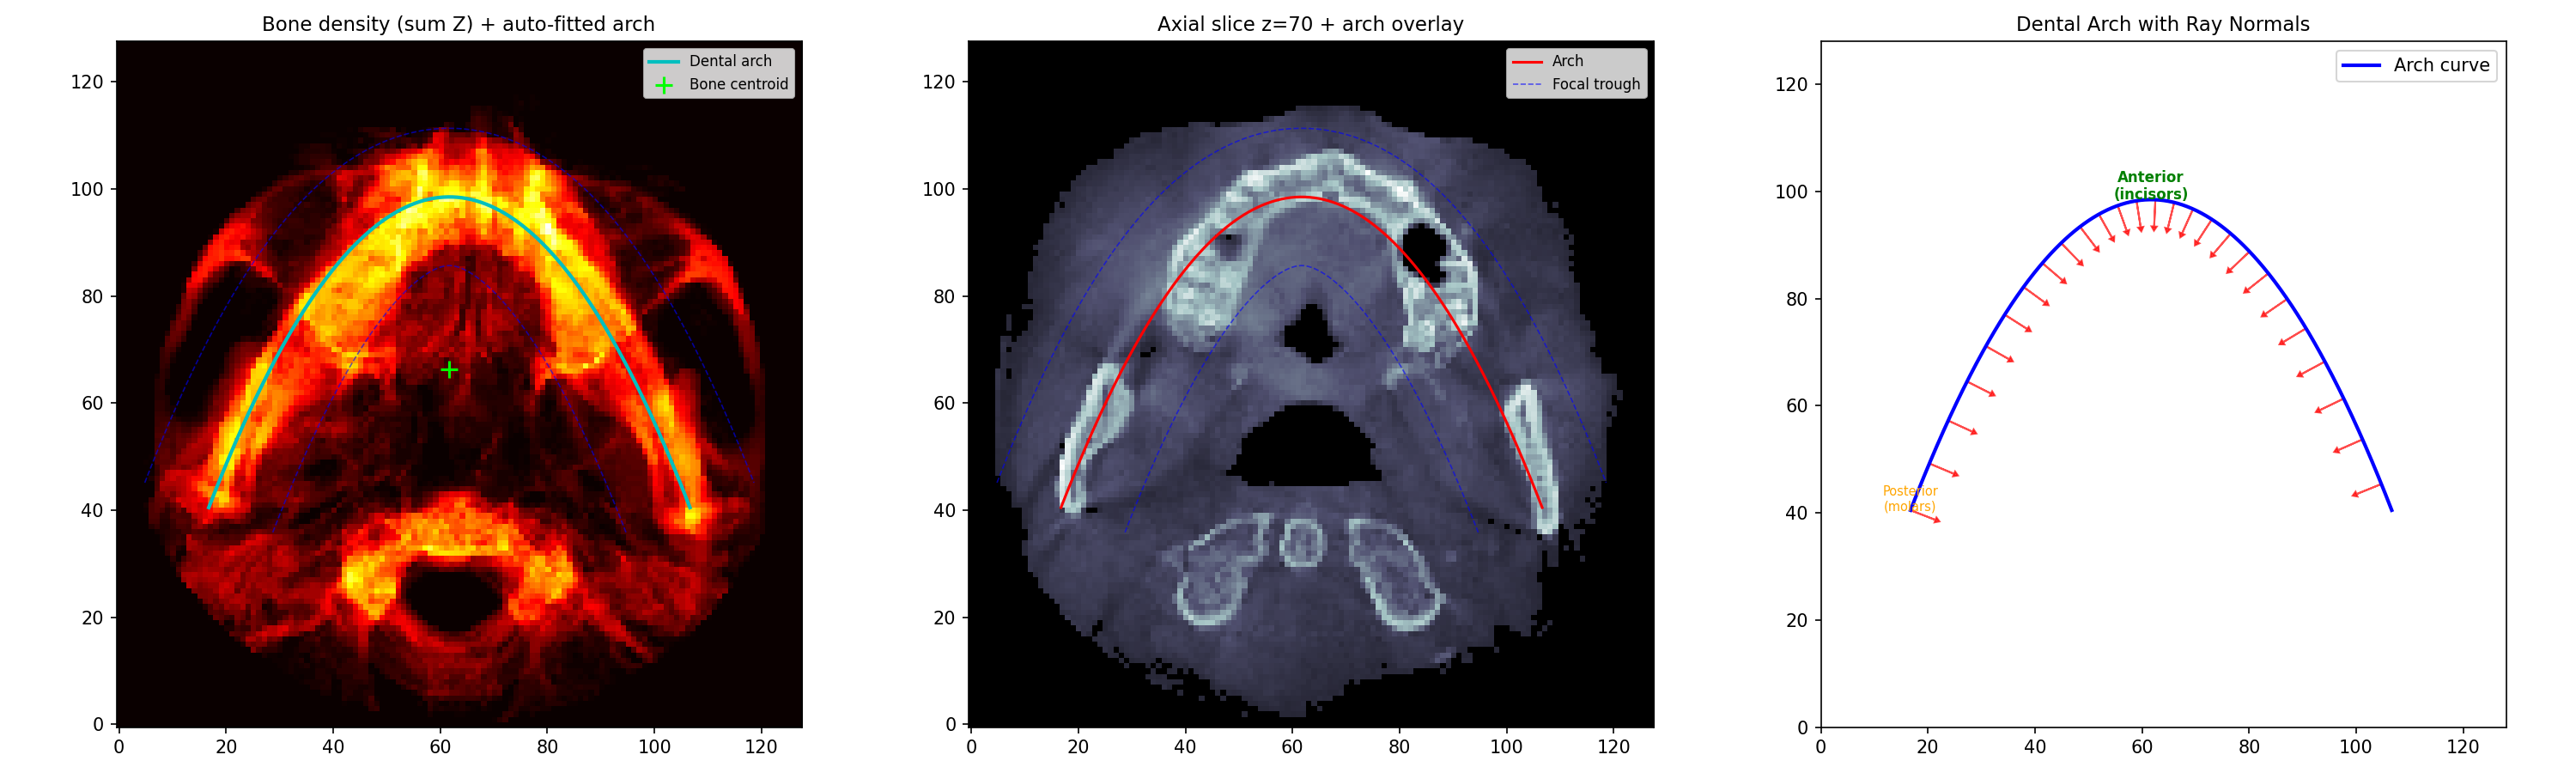
\includegraphics[width=0.48\textwidth]{dental_arch_geometry.png}
\caption{Dynamic patient-adaptive parabolic dental arch and focal-trough geometry derived from each CBCT volume. The bone-density projection of the dental Z-band (FIX1) is contrast-enhanced with CLAHE and thresholded; the AP band (FIX2) and largest connected component (FIX3) yield the bone mask from which the arch parameters $(c_x, c_y, w, d)$ are estimated. The fitted parabolic curve, focal-trough envelope, and per-column normal vectors used for ray casting are overlaid on the CBCT axial slice and the bone-density projection.}
\label{fig:arch_geom}
\end{figure}

\subsection{Curved-Focal-Trough DRR Rendering}

The panoramic DRR generator (\texttt{PanoramicDRRGenerator}) implements the curved-focal-trough projection model (Fig.~\ref{fig:ray_result}, Fig.~\ref{fig:ray_equations}). The output panoramic image has spatial dimensions of $512 \times 256$ pixels (width $\times$ height, i.e., panoramic arc length $\times$ vertical extent). The focal trough depth is 30.0\,mm, corresponding to $30.0 / 1.17 \approx 25.6$ voxels (using an approximate scale factor of 1.17\,mm/voxel for the $128^3$ normalized volume). The sampling grid contains $60$ depth samples, giving a step size of $\Delta\ell = 0.5$\,mm per step.

For each panoramic pixel $(u, v)$:
\begin{enumerate}
    \item The horizontal position $u$ selects a point on the arch curve and its inward normal vector $\mathbf{N}_u$.
    \item The vertical position $v$ defines the height within the CBCT volume.
    \item A ray of length equal to the focal-trough depth is cast along $\mathbf{N}_u$ through the 3D volume, sampling $D=60$ positions at equal intervals.
    \item At each sample position $\mathbf{x}_k$, the attenuation coefficient $\mu_k$ is obtained via trilinear interpolation of the preprocessed $128^3$ volume.
    \item The discrete Beer-Lambert line integral is accumulated:
    \begin{equation}
        A(u,v) \approx \sum_{k=1}^{D} \mu_k \,\Delta\ell.
        \label{eq:disc}
    \end{equation}
    \item The raw panoramic pixel value is computed as $P(u,v) = A(u,v)$ (the positive line integral, where higher values correspond to denser material).
\end{enumerate}

\begin{figure}[t]
\centering
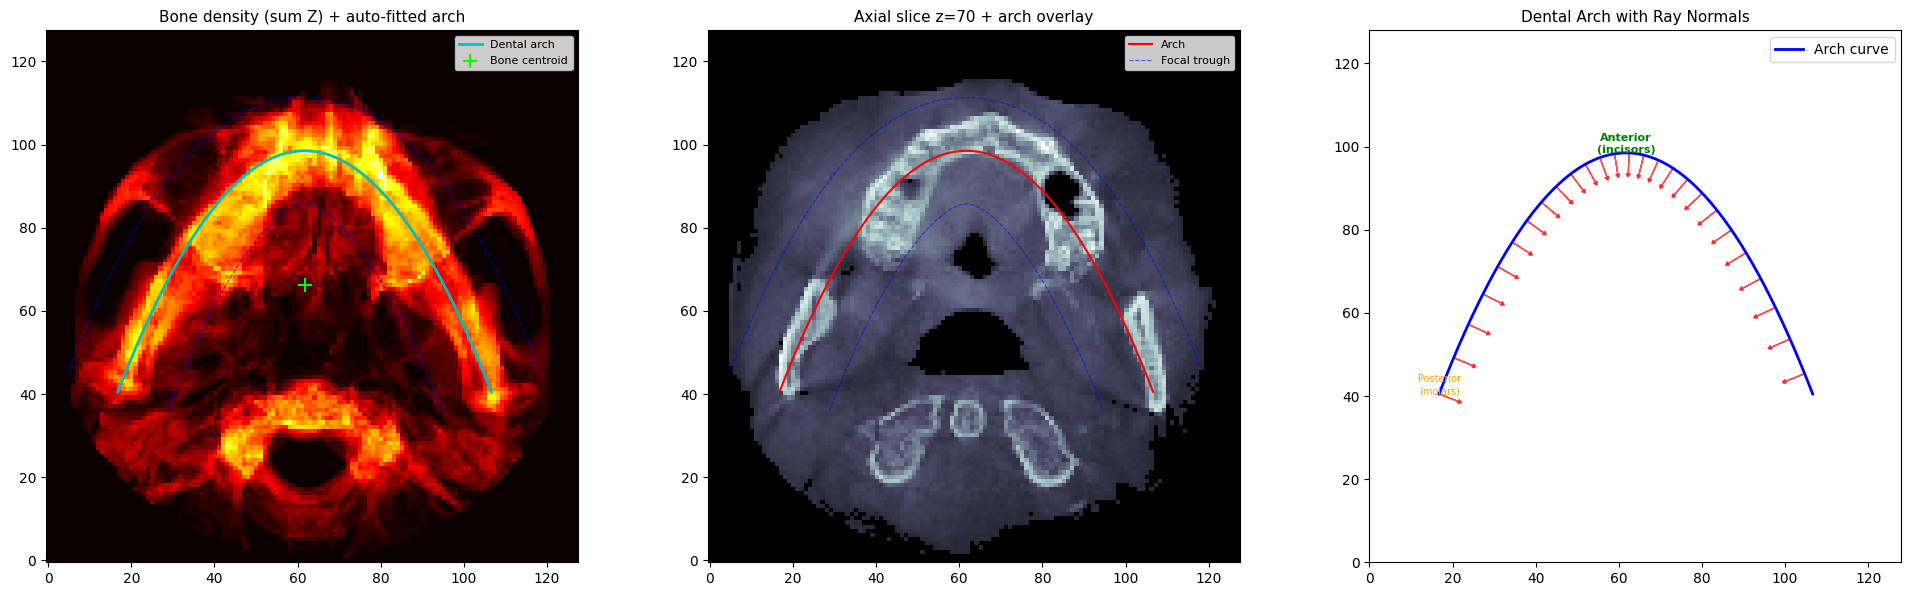
\includegraphics[width=0.48\textwidth]{ray_tracing_result.png}
\caption{Curved-arch ray tracing result showing the sampling behavior of the DRR projection through the focal trough. Each column of the panoramic image corresponds to one arch position and its associated normal ray.}
\label{fig:ray_result}
\end{figure}

\begin{figure}[t]
\centering
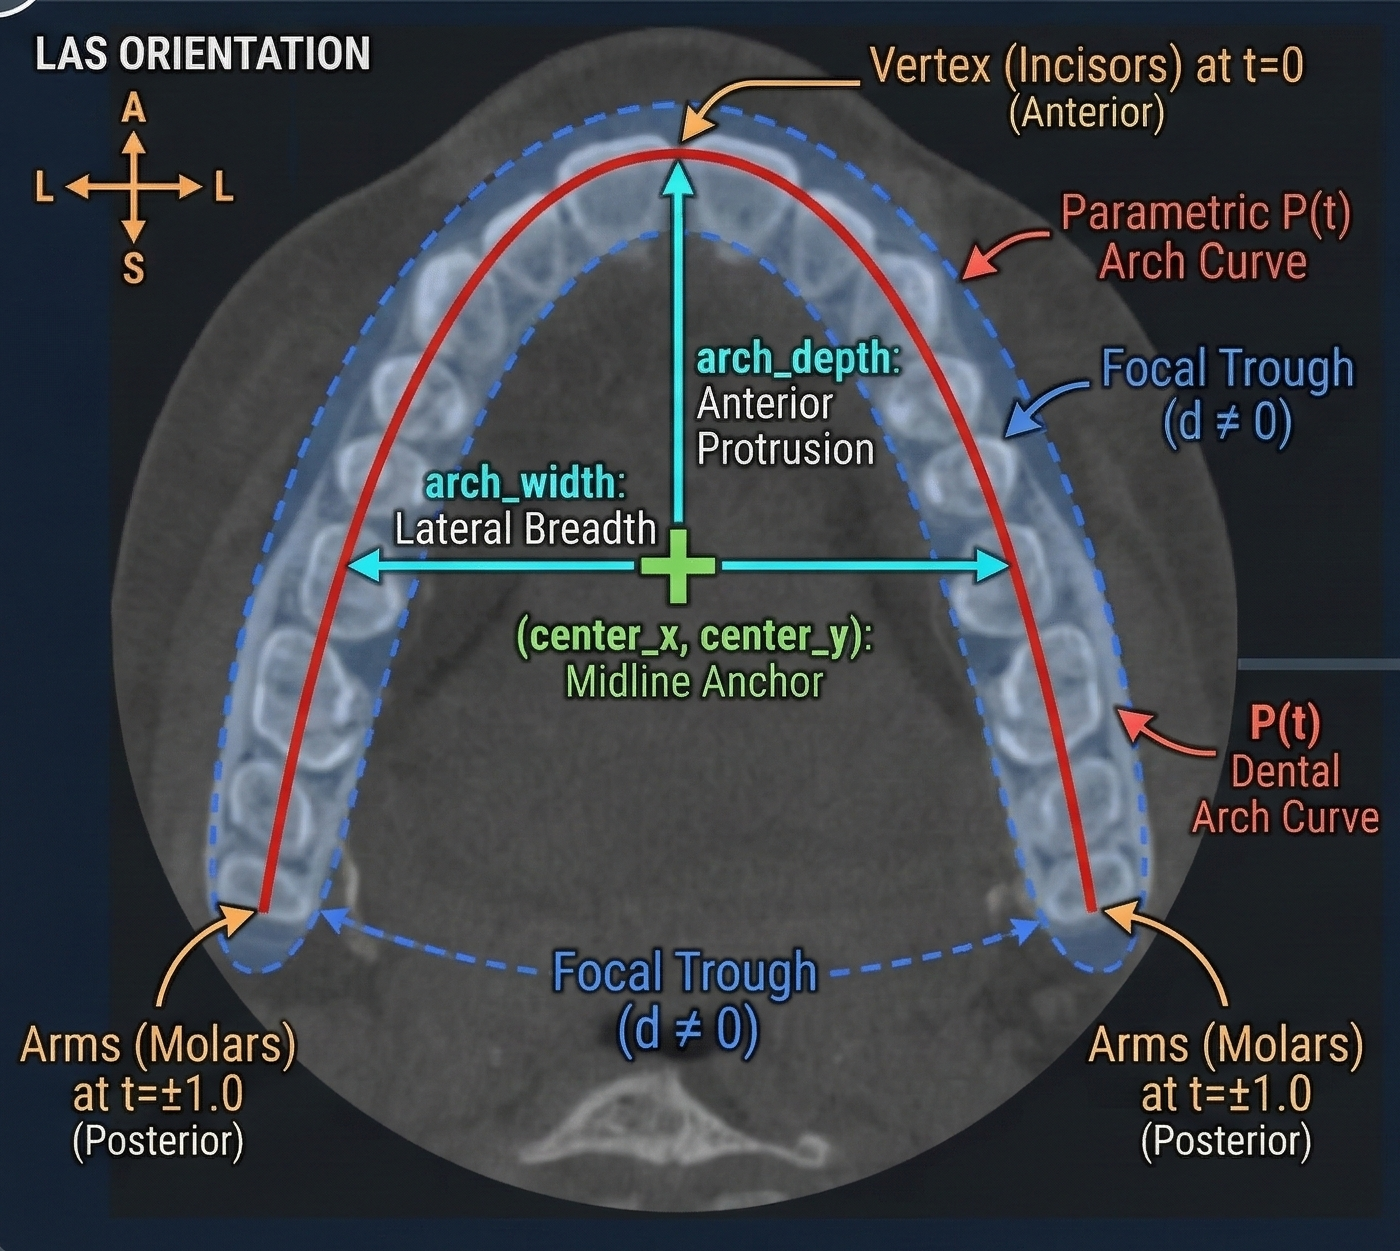
\includegraphics[width=0.48\textwidth]{Explained_Ray_tracing.png}
\caption{Equation-level and geometric interpretation of the curved focal-trough ray integration. Key components illustrated include: the tangent vector $\mathbf{T}_u$ along the arch, the normal vector $\mathbf{N}_u$ defining ray direction, the parametric arch curve P(t), arch width/depth parameters, and the LAS-orientation coordinate frame. The focal trough is shown as a band of nonzero depth $d \neq 0$ centered on the arch.}
\label{fig:ray_equations}
\end{figure}

\subsection{Radiographic Post-Processing}

The raw line-integral image is post-processed to improve radiographic realism and clinical interpretability:
\begin{enumerate}
    \item \textbf{Percentile windowing:} the 2nd and 98th percentiles of pixel intensities are used as the display window, suppressing outliers from dense metal artifacts.
    \item \textbf{Normalization:} the windowed image is linearly scaled to $[0, 1]$.
    \item \textbf{Gamma correction:} a gamma value of $\gamma = 0.8$ is applied to brighten mid-tones, approximating the appearance of clinical OPG film.
    \item \textbf{Unsharp masking:} a Gaussian-blurred version is subtracted from the normalized image to enhance high-frequency edge detail in tooth and bone boundaries.
\end{enumerate}
The resulting mean pixel value across all 21 volumes lies in the range $[0.631, 0.766]$, with full dynamic range $[0.0, 1.0]$, confirming that the post-processing produces consistently normalized outputs.

\subsection{Multi-View Augmentation and Dataset Packaging}
\label{subsec:aug}

To increase the diversity of the paired training set, each of the 21 preprocessed CBCT volumes is projected under three augmentation settings (Fig.~\ref{fig:rot_cmp}):
\begin{itemize}
    \item \textbf{Geometric augmentation:} the volume is rotated by $-3^\circ$, $0^\circ$ (identity), and $+3^\circ$ around the z-axis using SciPy \texttt{ndimage.rotate} (first-order interpolation, no reshape).
    \item \textbf{Intensity augmentation:} Poisson photon-counting noise is added with intensity parameter 1000.0, simulating quantum noise in X-ray detection. Random brightness and contrast jitter are applied with brightness offset $\in [-0.03, 0.03]$ and contrast scale drawn from a uniform distribution.
\end{itemize}

This produces $21 \times 3 = 63$ augmented panoramic--CBCT pairs. Each pair stores the panoramic image tensor, the volume index, the augmentation label, and the rotation angle. The full paired dataset is serialized as a PyTorch \texttt{.pt} file (\texttt{paired\_panoramic\_cbct\_dataset.pt}), containing: panoramic tensors of shape $[1, 256, 512]$, CBCT volume tensors of shape $[1, 128, 128, 128]$, and CBCT metadata dictionaries. The file size is 187.2\,MB. A \texttt{PairedPanoramicCBCTDataset} PyTorch \texttt{Dataset} class and \texttt{DataLoader} (batch size 1, 21 batches) wrap the dataset for training pipelines supporting batching, shuffling, and on-the-fly augmentation.

% =========================================================
\section{Loss Functions and Quality Metrics}
\label{sec:loss}
% =========================================================

\subsection{Individual Metrics}

Four quality metrics are computed for every panoramic DRR pair:
\begin{itemize}
    \item \textbf{L1 (MAE):} pixel-wise mean absolute error, measuring the average per-pixel deviation.
    \item \textbf{MSE (L2):} pixel-wise mean squared error, more sensitive to large deviations.
    \item \textbf{SSIM:} structural similarity index computed with a Gaussian kernel ($\sigma=1.5$, window size 11), capturing luminance, contrast, and structural fidelity. Implemented as a differentiable 2D module (\texttt{SSIMLoss2D}) using constants $C_1 = 0.0001$, $C_2 = 0.0009$.
    \item \textbf{PSNR:} peak signal-to-noise ratio (dB), defined as $10\log_{10}(1/\text{MSE})$, providing a logarithmic measure of signal fidelity.
\end{itemize}

\subsection{Combined Training Loss}

A weighted combined loss function is defined for training downstream networks:
\begin{equation}
\mathcal{L} = \alpha \cdot L_1 + \beta \cdot (1 - \text{SSIM}) + \gamma \cdot L_\text{MSE},
\label{eq:loss}
\end{equation}
with weights $\alpha=1.0$, $\beta=5.0$, $\gamma=1.0$. The higher weight on SSIM loss encourages structural fidelity rather than purely pixel-wise accuracy, which is appropriate for medical image synthesis tasks where perceptual and structural quality are clinically relevant.

\subsection{Evaluation Protocol}

Two complementary evaluations are performed:

\textbf{Round-trip self-consistency:} Each CBCT volume in the DataLoader is re-projected through the DRR generator and the resulting panoramic is compared against the stored panoramic from the same volume. This measures the DRR generator's internal consistency (i.e., deterministic projection reproducibility). Round-trip metrics are L1\,=\,0, SSIM\,=\,1.0, PSNR\,=\,$\infty$, confirming exact self-consistency.

\textbf{Cross-view augmentation quality:} Augmented panoramics from the three rotation settings are compared against the identity ($0^\circ$) panoramic of the corresponding volume. This measures the sensitivity of the projection to small patient-position variations. Table~\ref{tab:metrics} reports representative aggregated values. Full per-volume, per-augmentation results are detailed in the notebook output.

% =========================================================
\section{Experimental Results}
\label{sec:results}
% =========================================================

\subsection{Output Inventory}

The complete pipeline execution on 21 CBCT volumes produced the following artifacts:
\begin{itemize}
    \item 21 synthetic panoramic DRR images (PNG), one per volume, saved to \texttt{project/output/}.
    \item 63 augmented panoramic images (PNG), saved to \texttt{project/output/augmented/}.
    \item One paired PyTorch dataset file: \texttt{paired\_panoramic\_cbct\_dataset.pt} (187.2\,MB).
    \item Diagnostic visualization outputs: arch geometry figure, panoramic grid, quality verification panel, CBCT-to-panoramic comparison figure, paired CBCT--PX samples figure.
\end{itemize}

Average generation time per volume was 2.23 seconds on CPU, confirming the pipeline's practicality for offline dataset construction.

\subsection{Quantitative Results}

\begin{table}[t]
\caption{Quantitative Summary: Cross-View Quality Metrics with Dynamic Patient-Adaptive Arch}
\label{tab:metrics}
\centering
\begin{tabular}{l c c c}
\toprule
\textbf{Augmentation} & \textbf{Avg L1} & \textbf{Avg SSIM} & \textbf{Avg PSNR (dB)} \\
\midrule
rot+0deg (identity)   & 0.02687 & 0.7467 & 29.70 \\
rot$-$3deg            & 0.06714 & 0.5289 & 19.72 \\
rot+3deg              & 0.06995 & 0.5260 & 19.52 \\
\midrule
\multicolumn{4}{l}{\textit{Additional pipeline statistics:}} \\
\multicolumn{2}{l}{Processed CBCT volumes} & \multicolumn{2}{c}{21} \\
\multicolumn{2}{l}{Augmented panoramic variants} & \multicolumn{2}{c}{63} \\
\multicolumn{2}{l}{Dataset file size} & \multicolumn{2}{c}{187.2\,MB} \\
\multicolumn{2}{l}{Avg generation time/volume} & \multicolumn{2}{c}{2.23\,s (CPU)} \\
\bottomrule
\end{tabular}
\end{table}

The rot+0deg results (L1\,=\,0.02687, SSIM\,=\,0.7467, PSNR\,=\,29.70\,dB) reflect cross-volume consistency when the identity augmentation is compared against itself for the dynamic patient-adaptive arch, confirming stable and repeatable DRR generation. The $\pm3^\circ$ rotation conditions show expected degradation (SSIM drops to $\approx$0.52, PSNR to $\approx$19.5--19.7\,dB), consistent with meaningful geometric shift between views. These numbers establish the practical operating range of the augmentation strategy under per-patient arch fitting.

\subsection{Visual Results}

Fig.~\ref{fig:cbct_to_pan} shows representative CBCT axial and coronal slices alongside the corresponding synthetic panoramic DRR, illustrating that dental structures (tooth crowns, roots, mandibular canal) are visually preserved in the projection.

\begin{figure}[t]
\centering
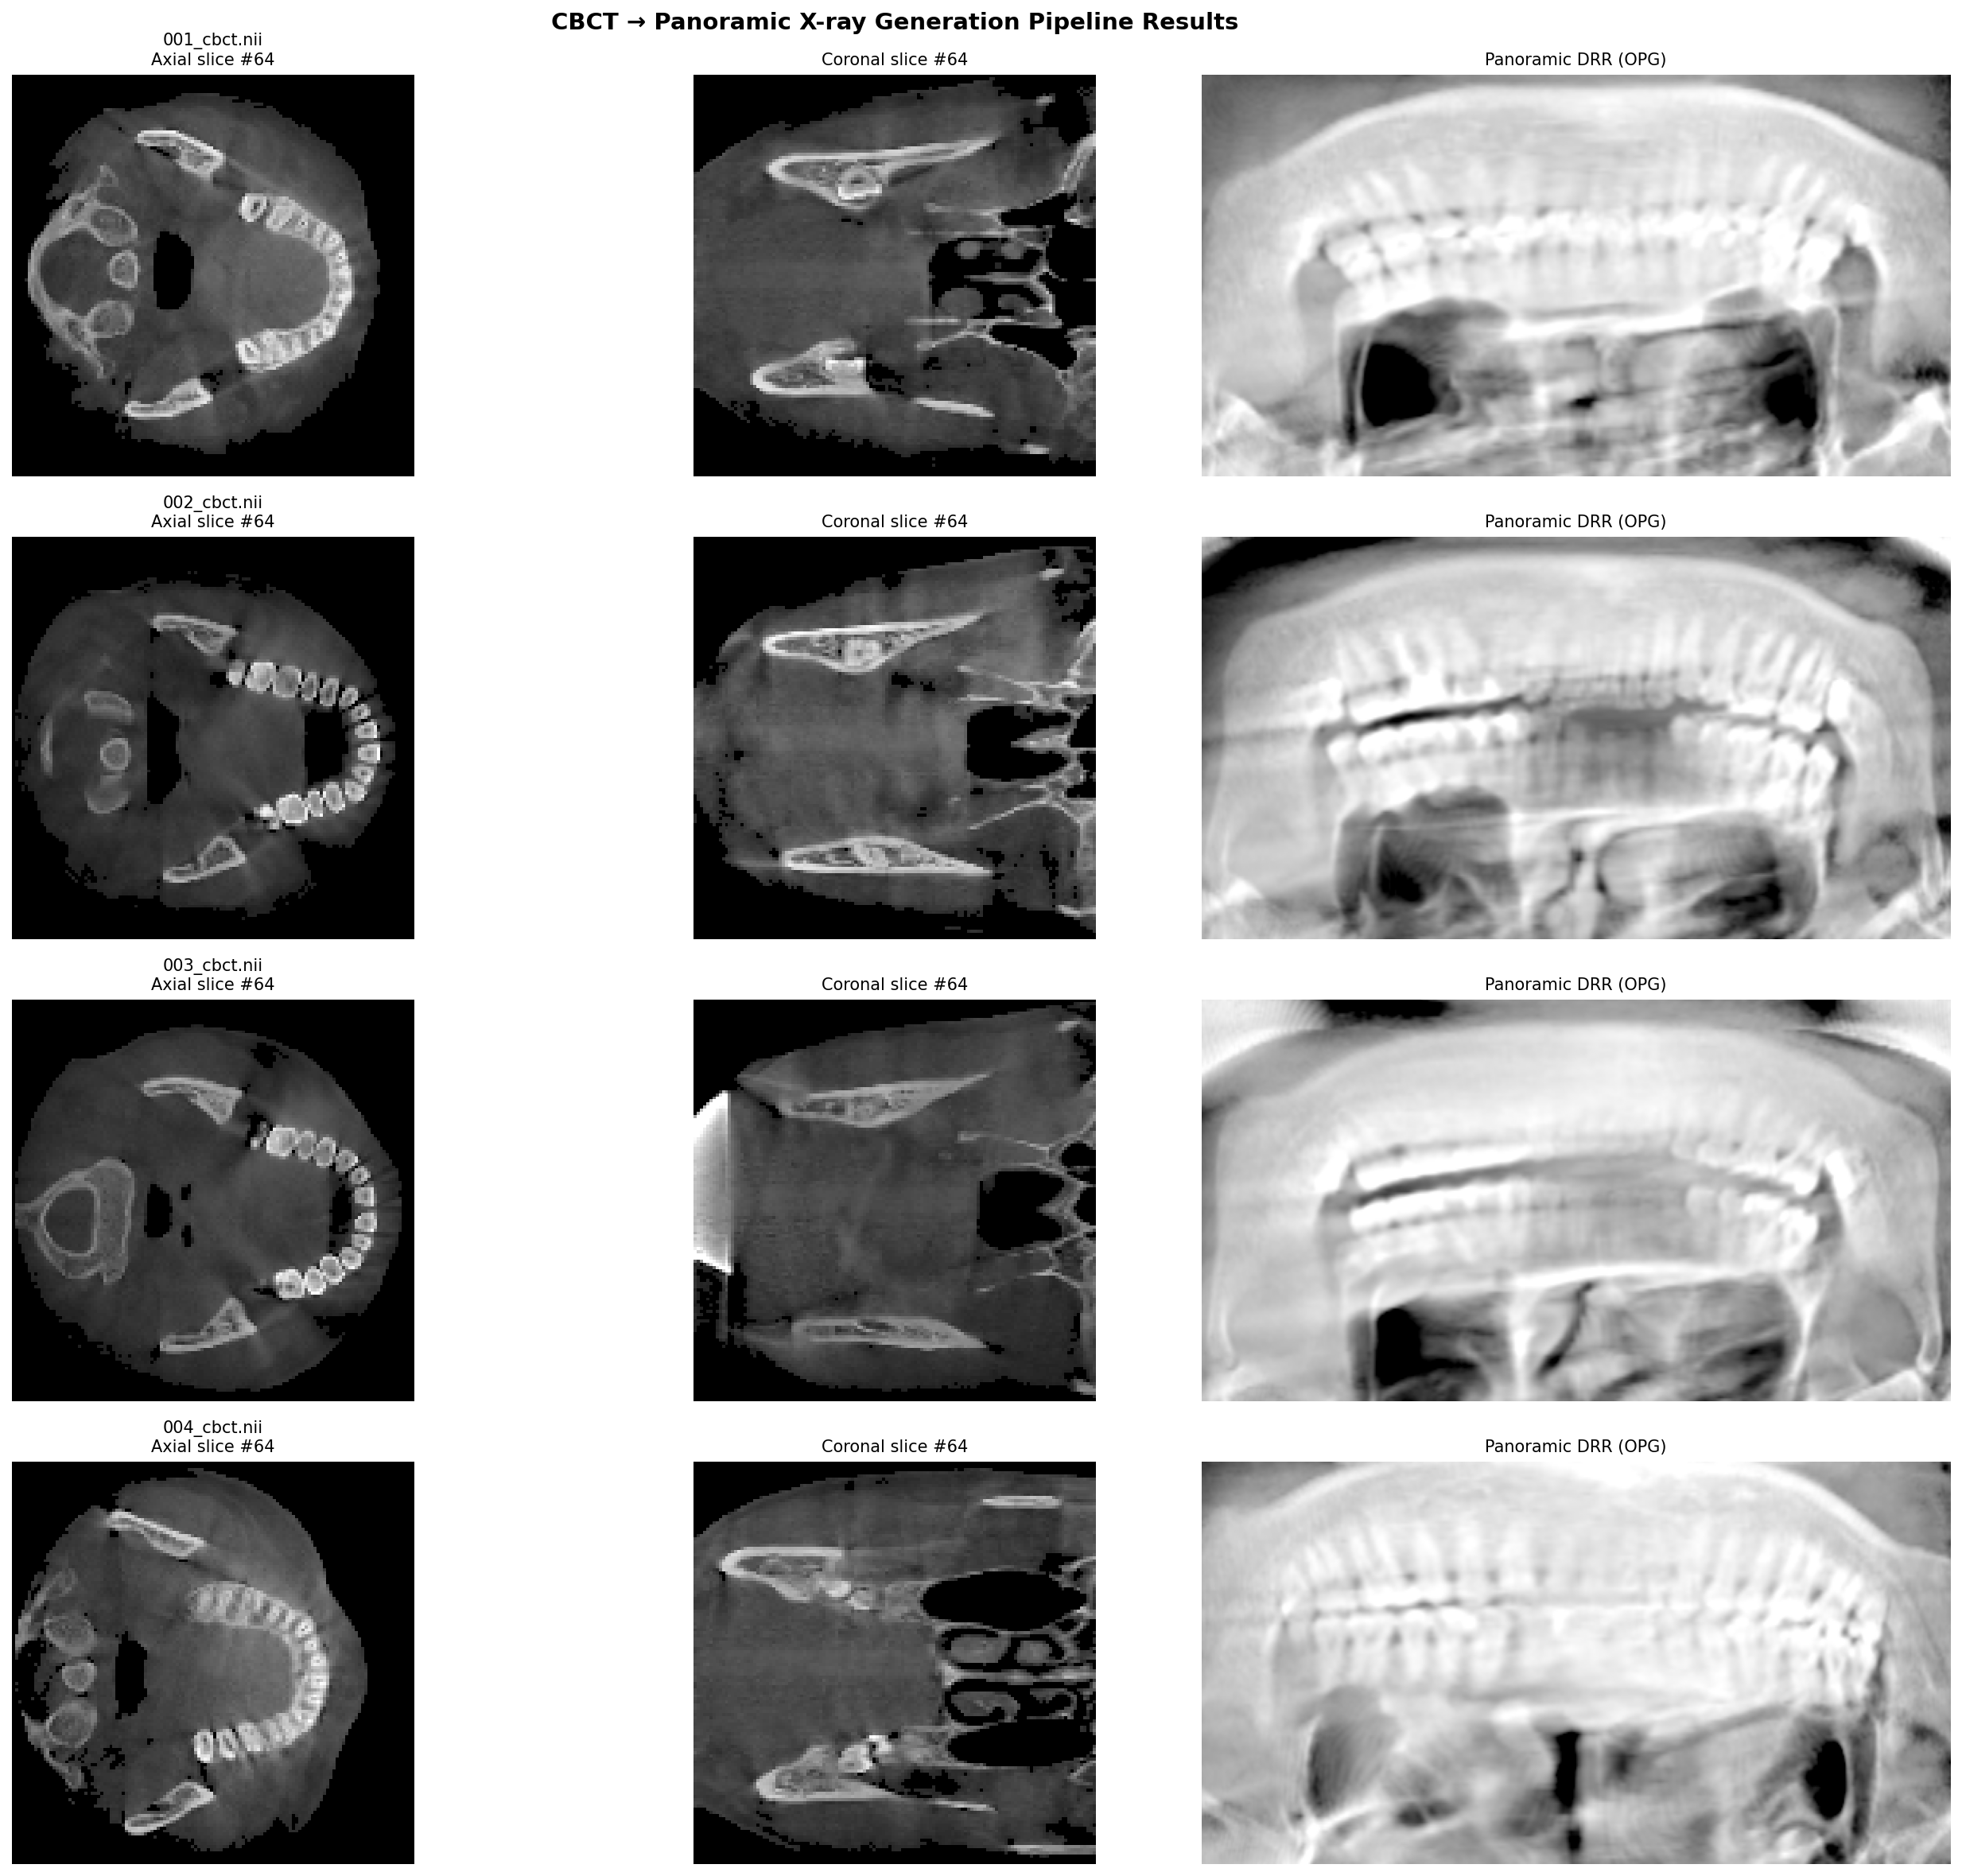
\includegraphics[width=0.48\textwidth]{cbct_to_panoramic_comparison.png}
\caption{Representative CBCT-to-panoramic visualization. Left and center: axial and coronal slices from a preprocessed CBCT volume at mid-depth (slice \#64). Right: the corresponding synthetic panoramic DRR (OPG) generated by the curved-arch Beer-Lambert pipeline.}
\label{fig:cbct_to_pan}
\end{figure}

Fig.~\ref{fig:pan_grid} presents a $2\times3$ grid of synthetic panoramic DRRs from the first six CBCT volumes, demonstrating consistent output quality and visual appearance across subjects.

\begin{figure}[t]
\centering
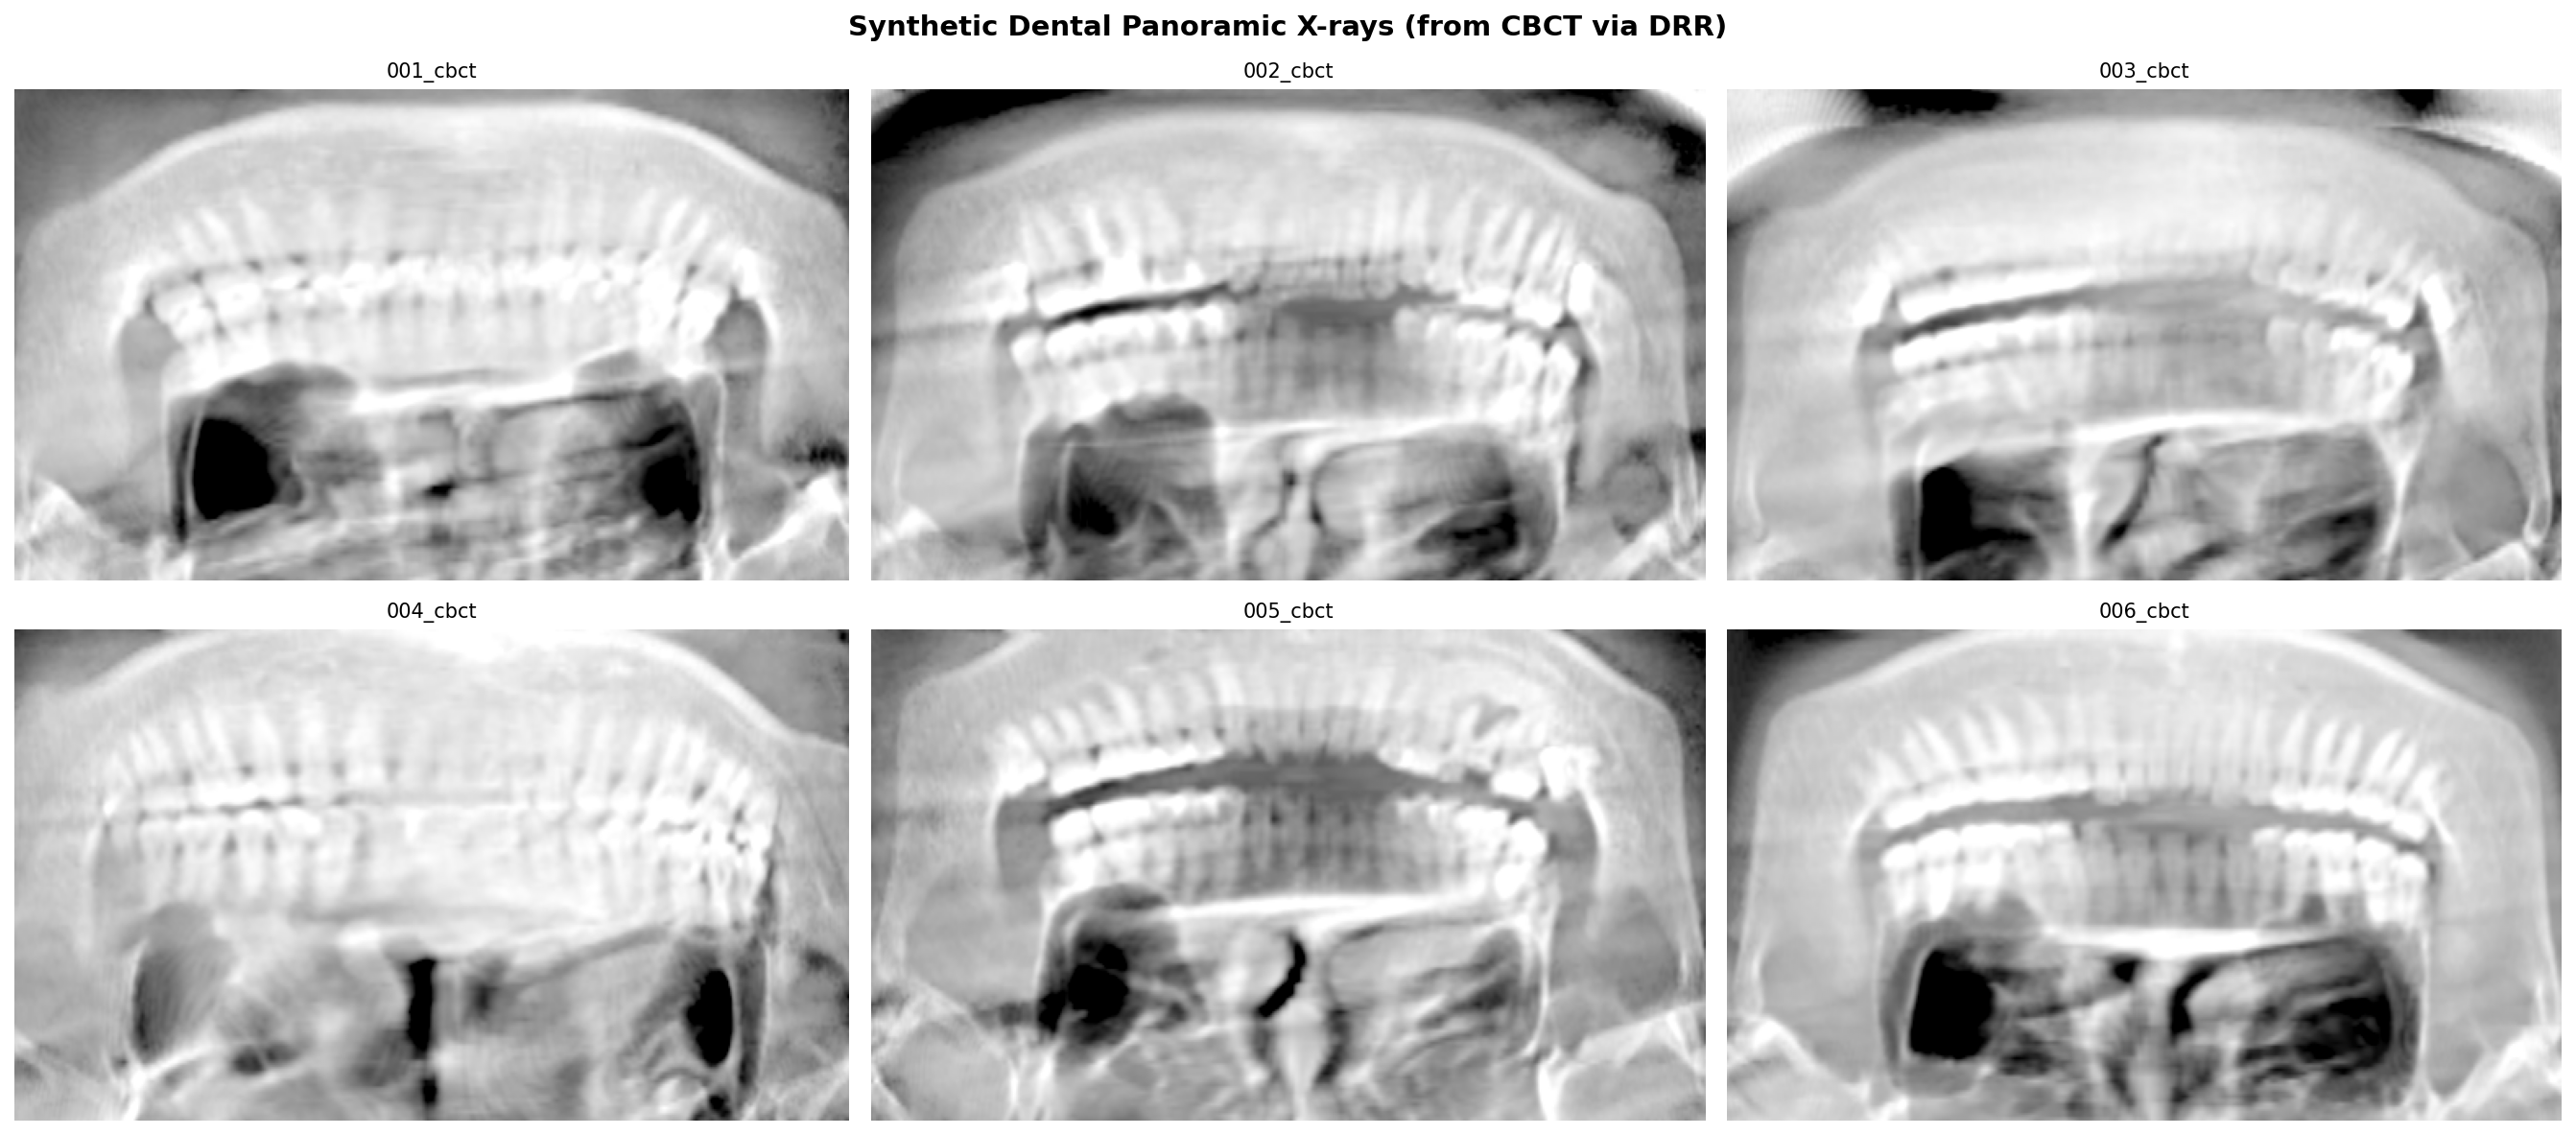
\includegraphics[width=0.48\textwidth]{panoramic_grid.png}
\caption{Grid of six synthetic panoramic X-rays generated from CBCT volumes 001--006. All images were generated with identical pipeline parameters, demonstrating consistent rendering quality across different patients with varying bone density and dentition.}
\label{fig:pan_grid}
\end{figure}

Fig.~\ref{fig:rot_cmp} illustrates the three augmented views for a representative volume, showing the expected geometric displacement between the $-3^\circ$, $0^\circ$, and $+3^\circ$ rotation conditions.

\begin{figure}[t]
\centering
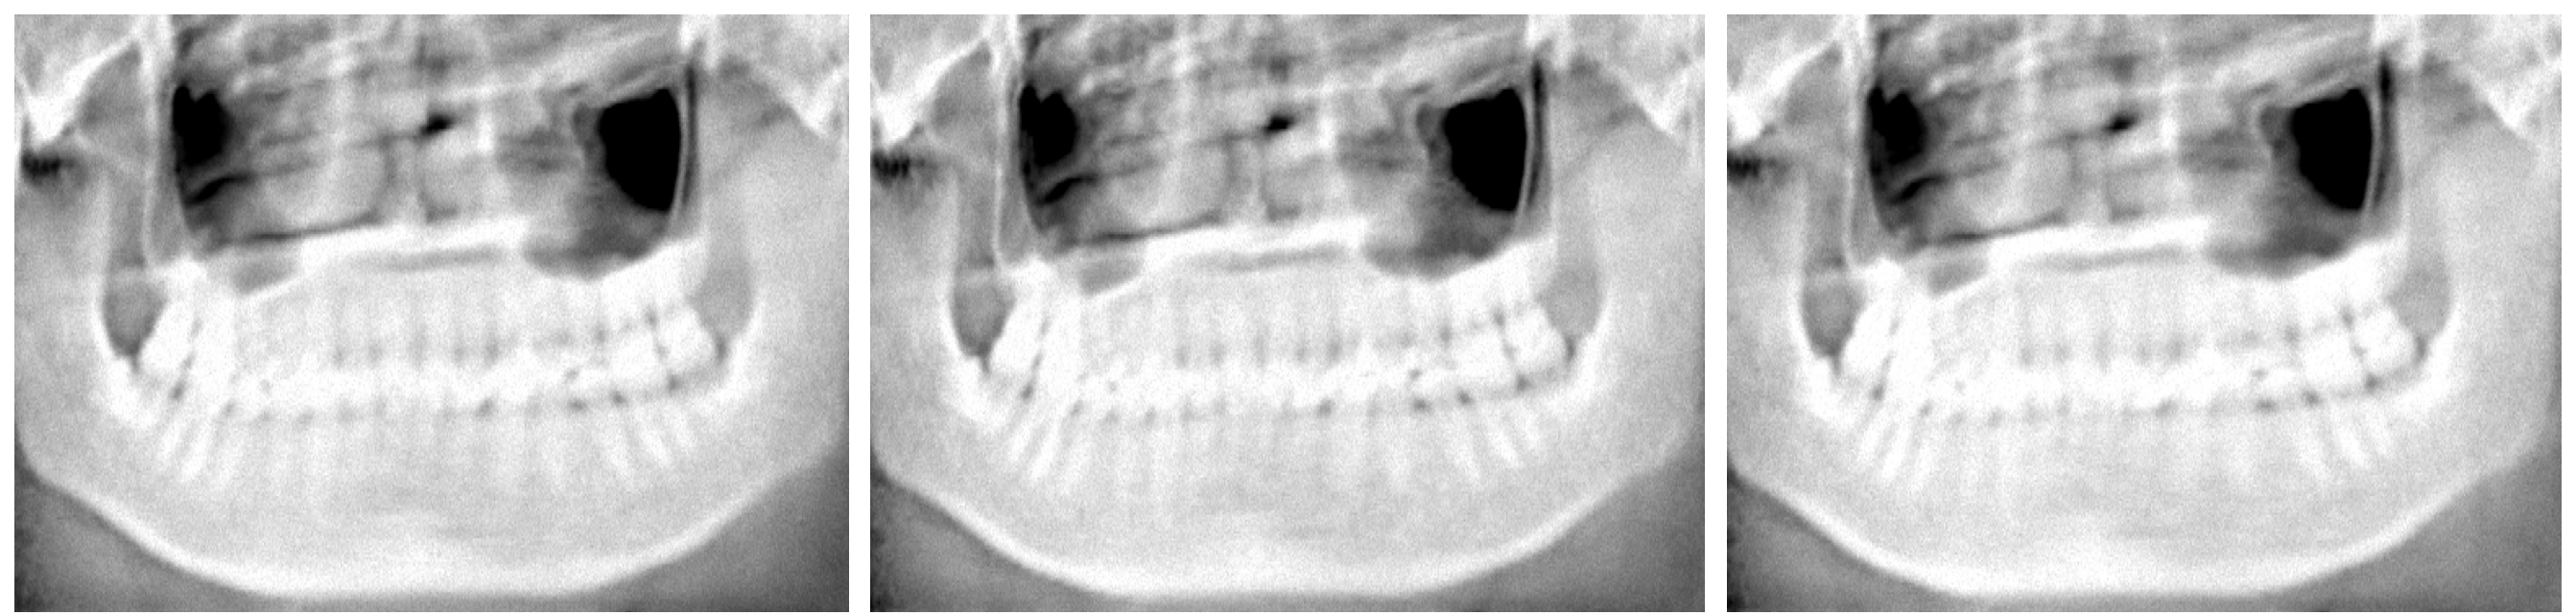
\includegraphics[width=0.48\textwidth]{rotation_comparison_minus3_0_plus3.png}
\caption{Multi-view augmentation outputs for a representative CBCT volume at rotation offsets of $-3^\circ$ (left), $0^\circ$ (center), and $+3^\circ$ (right). The $\pm3^\circ$ perturbations introduce visible geometric displacement in the panoramic arc, simulating slight patient-positioning variation.}
\label{fig:rot_cmp}
\end{figure}

Fig.~\ref{fig:paired_samples} shows examples of paired CBCT slices (axial, coronal, sagittal) alongside their corresponding synthetic panoramic DRRs from the exported \texttt{.pt} dataset, confirming the pairing integrity.

\begin{figure}[t]
\centering
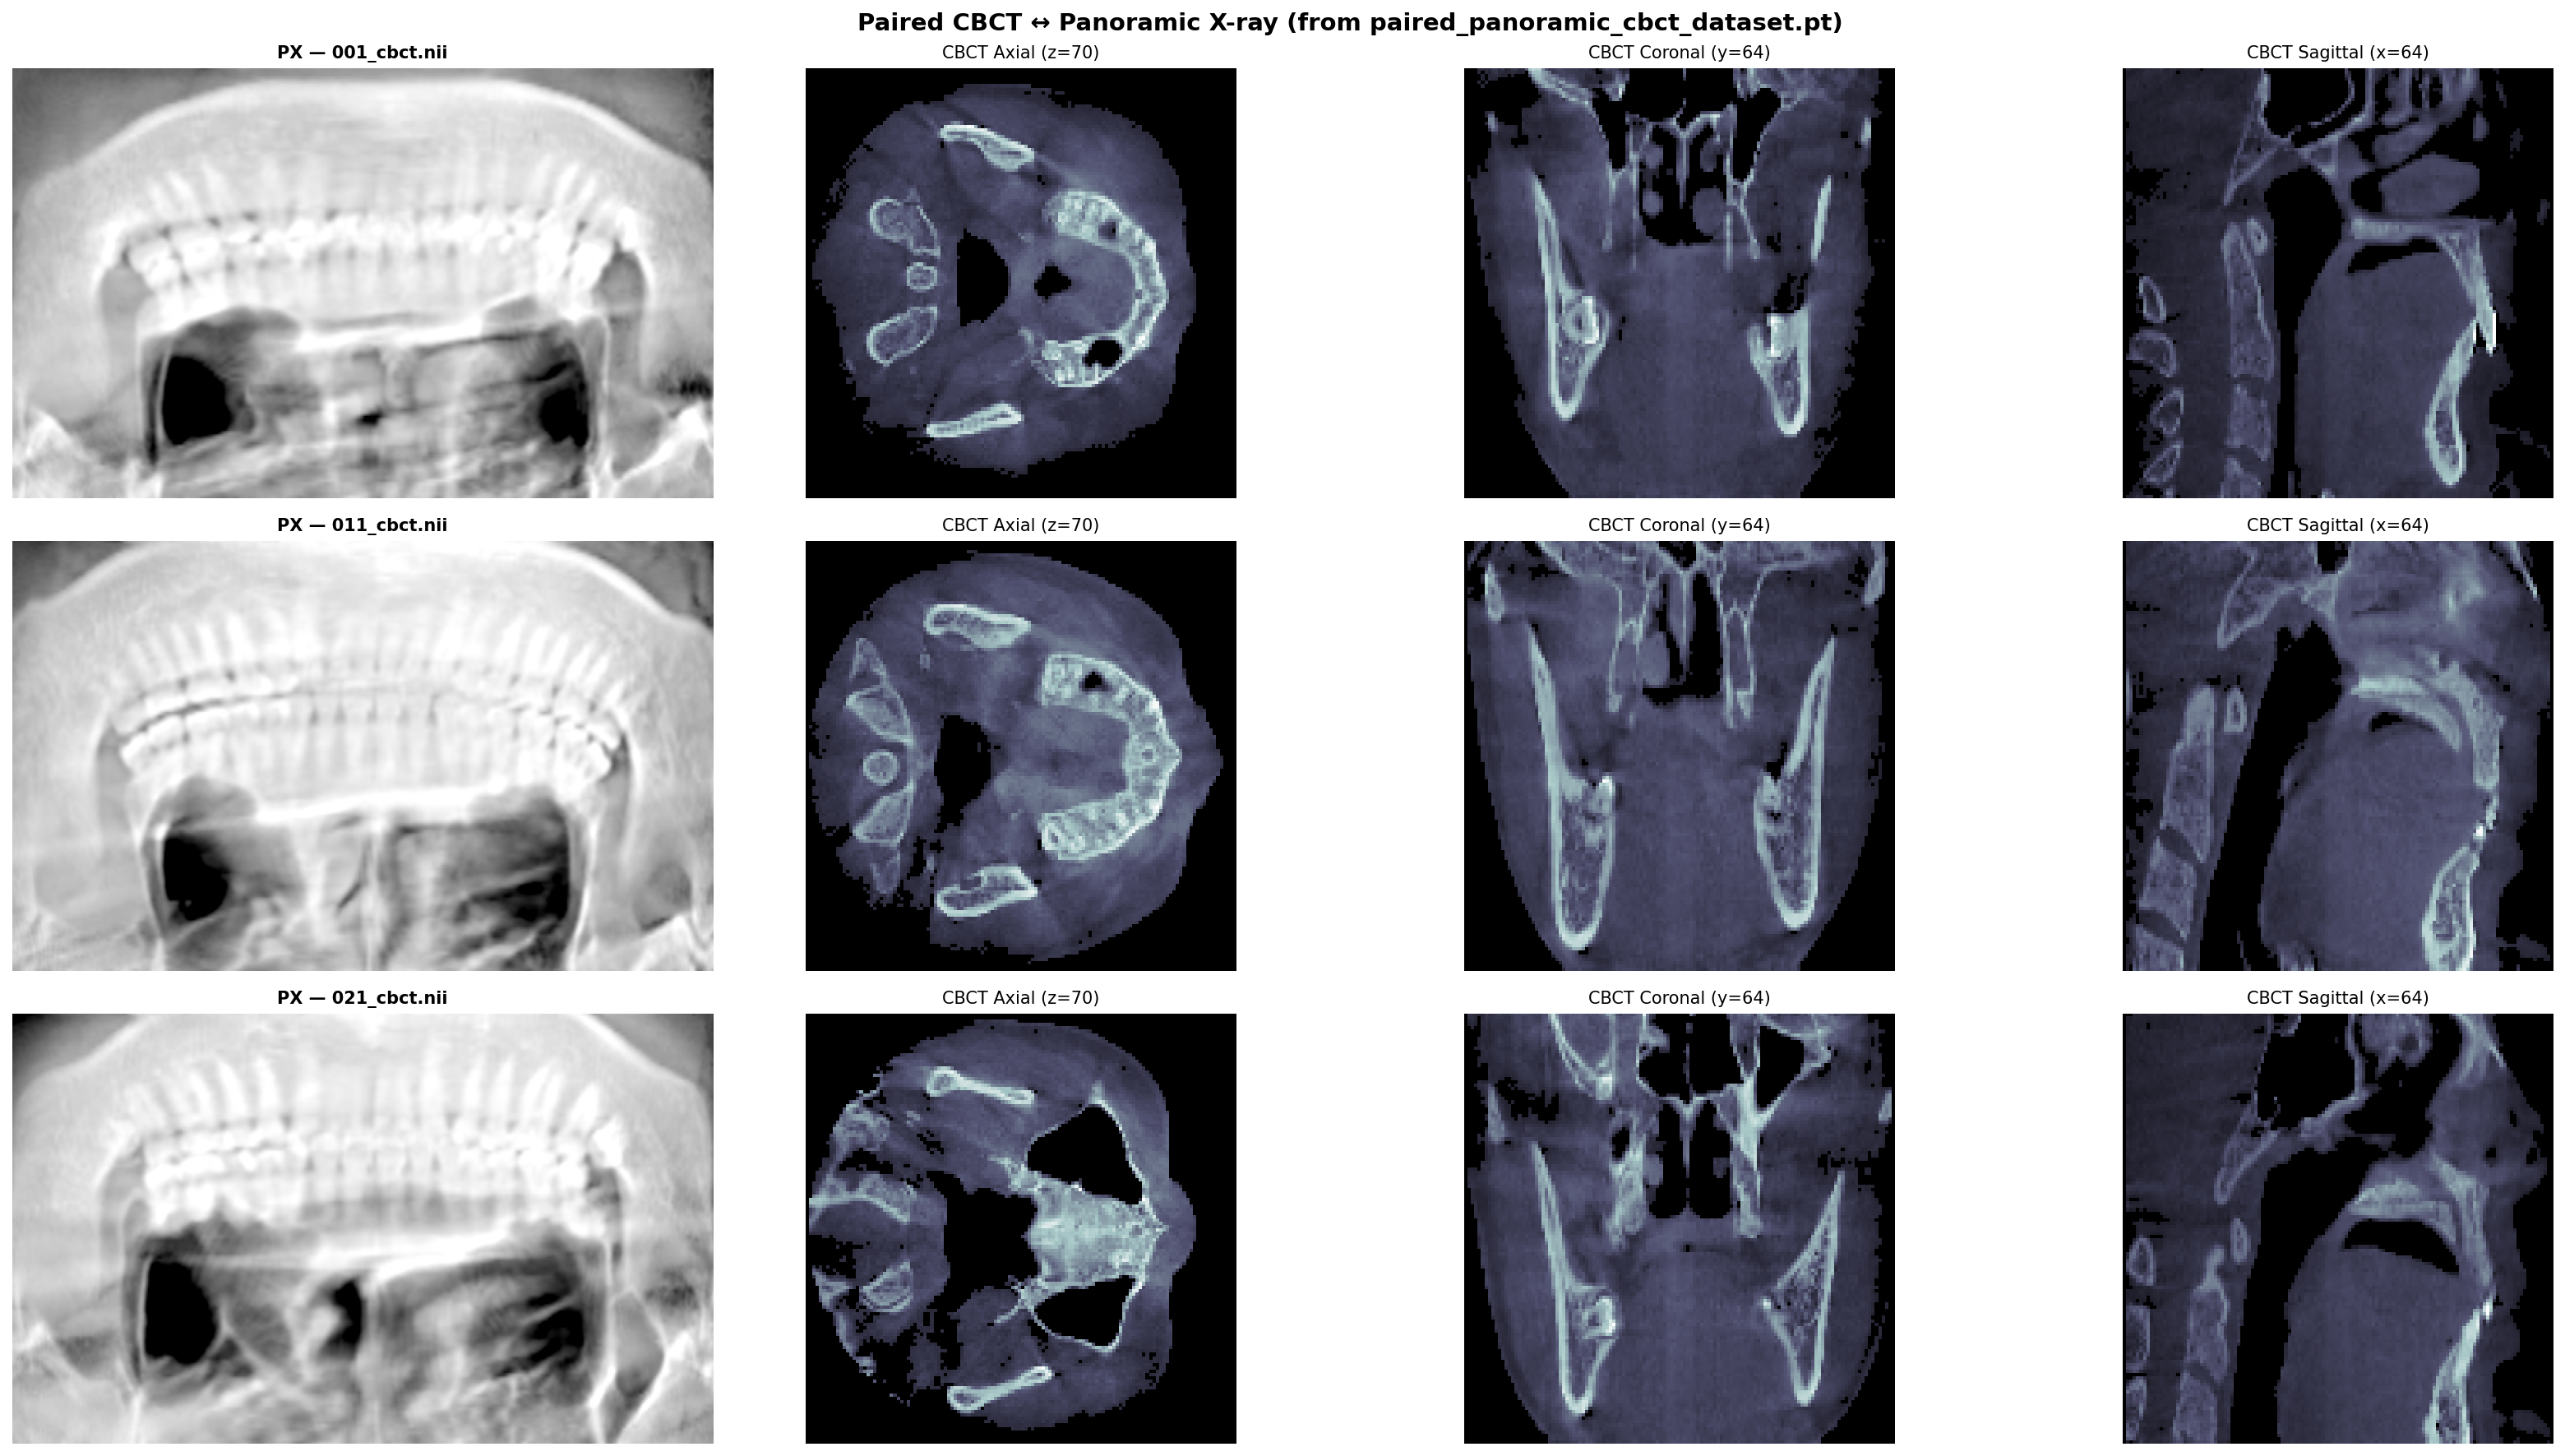
\includegraphics[width=0.48\textwidth]{paired_cbct_px_samples.png}
\caption{Examples of paired CBCT--panoramic X-ray (PX) samples from the exported \texttt{paired\_panoramic\_cbct\_dataset.pt}. Each row shows the panoramic DRR (column 1), CBCT axial slice (column 2), CBCT coronal slice (column 3), and CBCT sagittal slice (column 4) for the same volume, confirming pairing consistency.}
\label{fig:paired_samples}
\end{figure}

Fig.~\ref{fig:quality} presents the quality verification panel. Pixel distribution histograms show consistent bell-shaped distributions (mean pixel 0.702\,$\pm$\,0.037, std 0.217\,$\pm$\,0.021, contrast 0.312\,$\pm$\,0.043, dark fraction 2.7\,$\pm$\,1.4\%, bright fraction 16.6\,$\pm$\,5.5\%). All 21 images passed automated quality checks for dynamic range and contrast.

\begin{figure}[t]
\centering
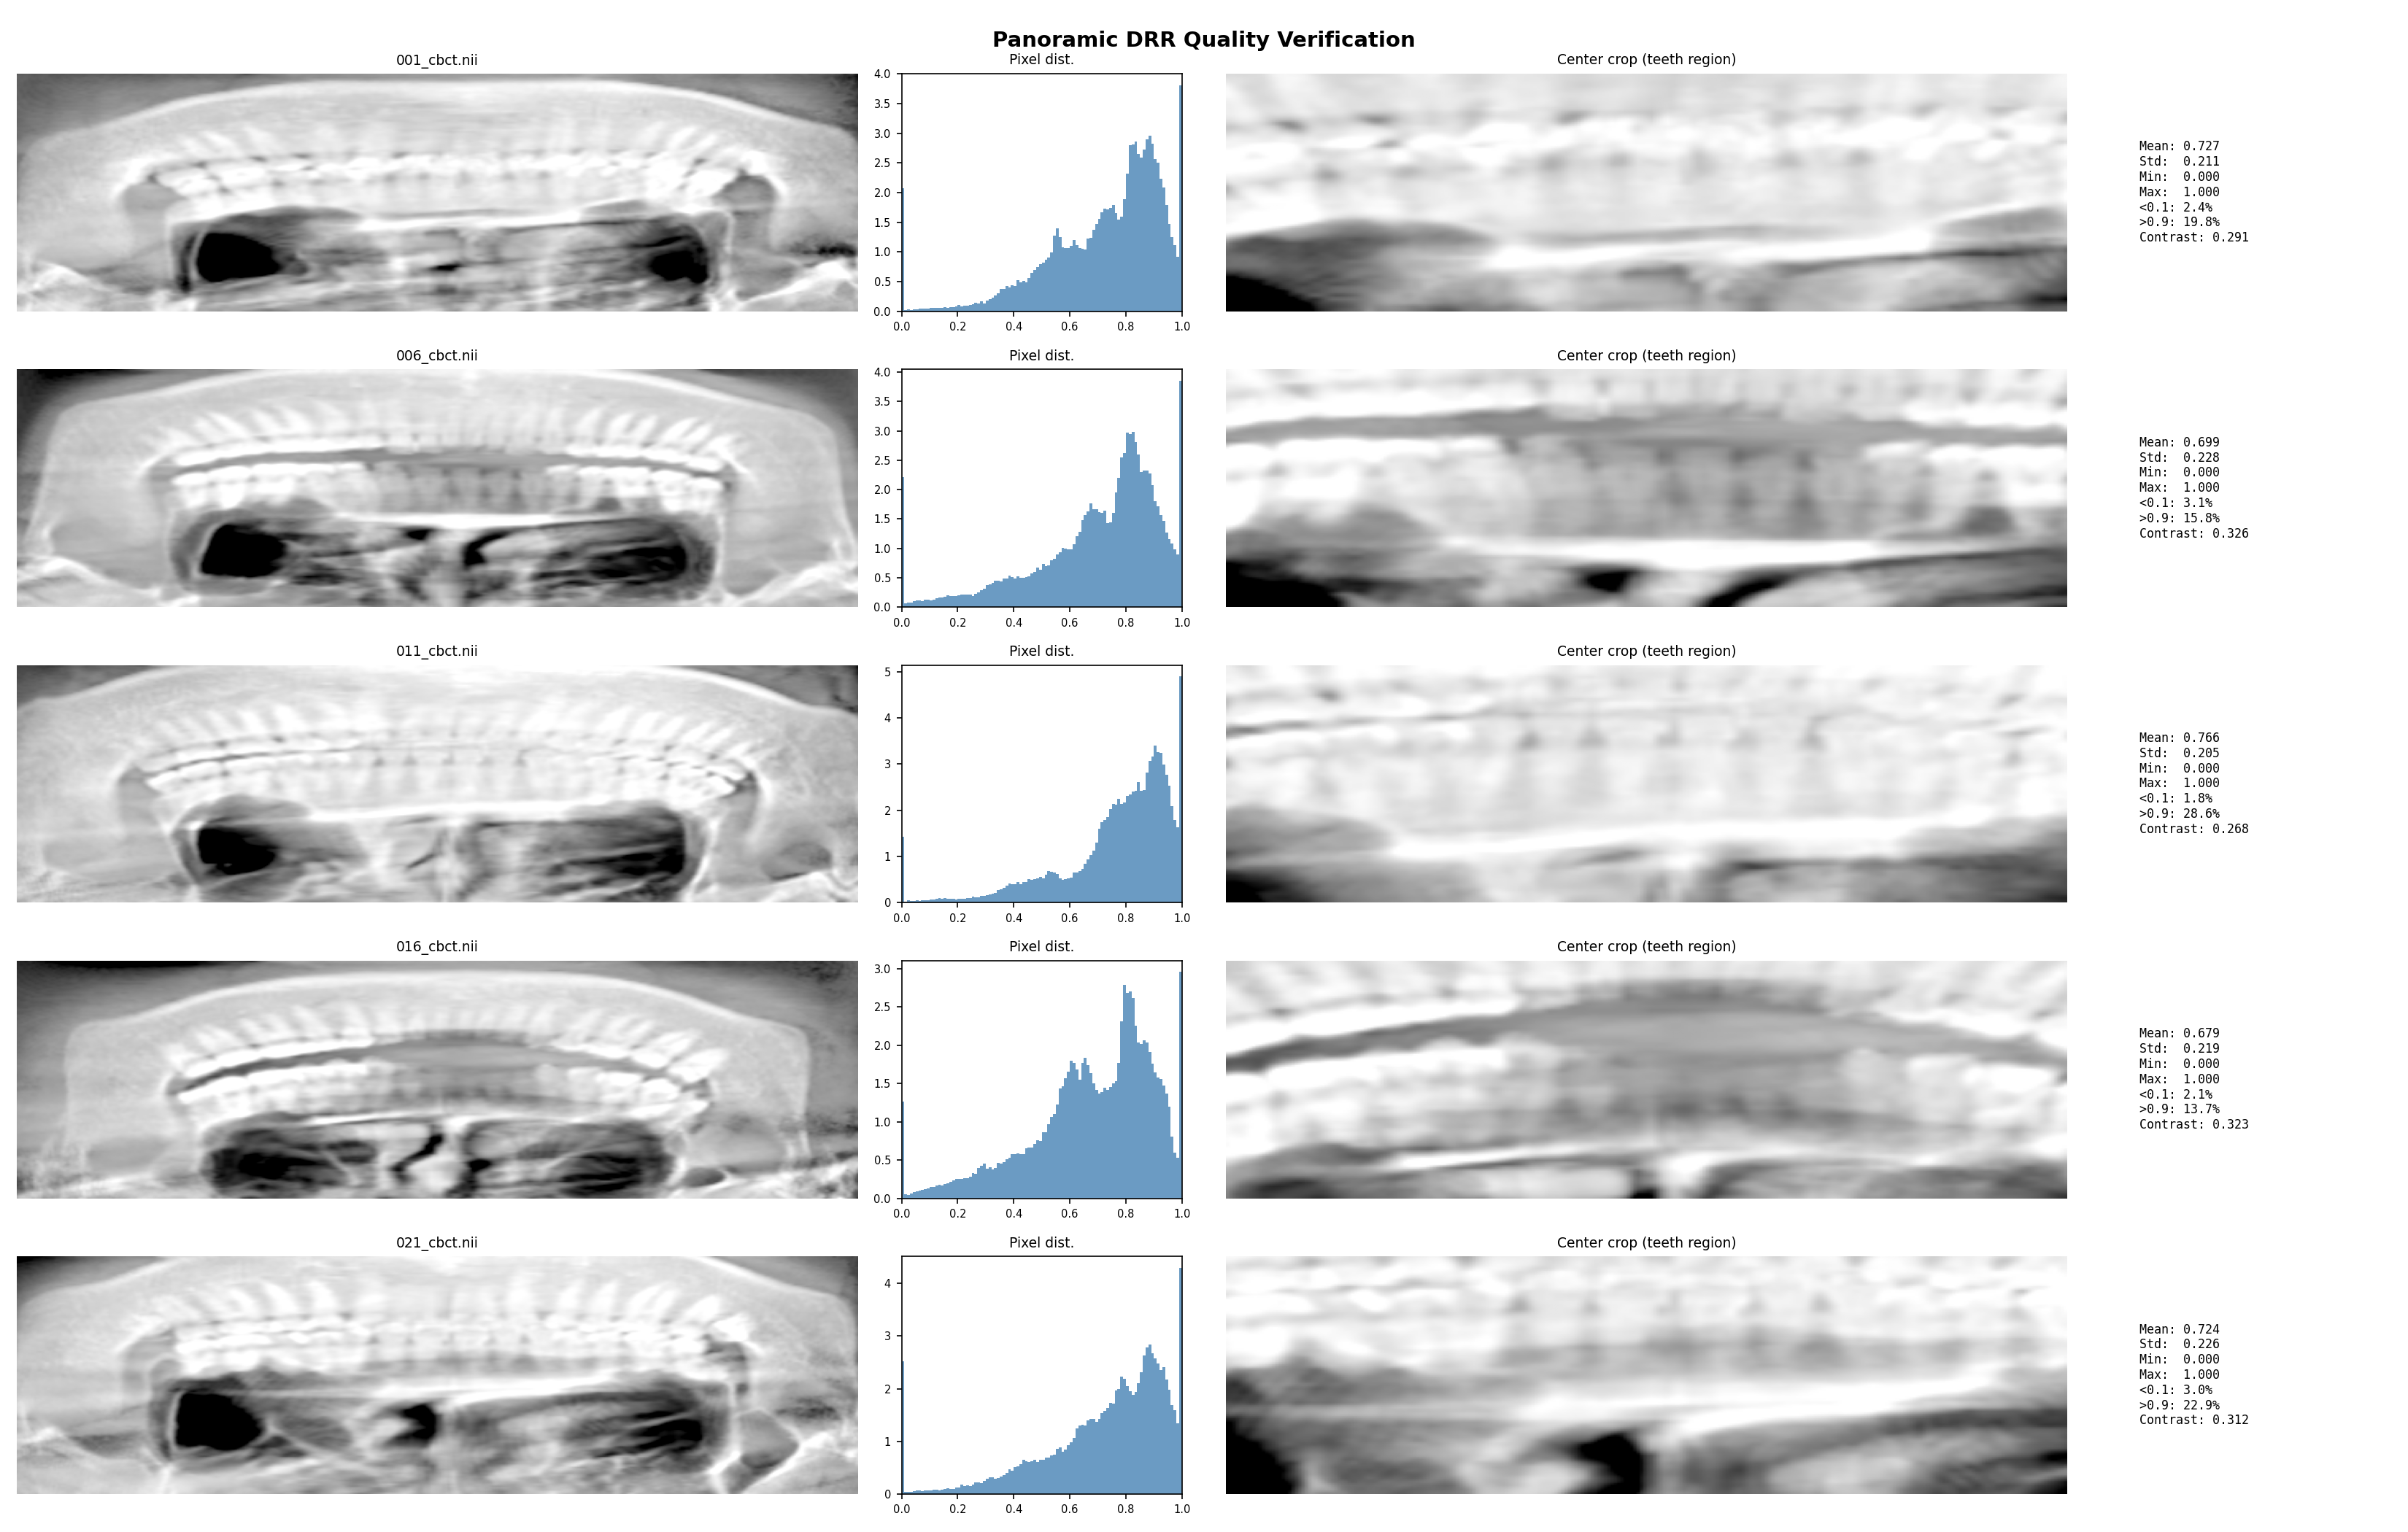
\includegraphics[width=0.48\textwidth]{quality_verification.png}
\caption{Quality verification panel for five representative synthetic panoramic DRRs (volumes 001, 006, 011, 016, 021). Each row shows the full panoramic image, its pixel histogram, a center crop of the teeth region, and per-image statistics (mean, std, min, max, contrast). All images passed dynamic range and contrast quality checks.}
\label{fig:quality}
\end{figure}

Fig.~\ref{fig:nebla_vs_ours} provides a visual comparison between the NeBLa reference approach and the panoramic outputs generated by the proposed pipeline.

\begin{figure*}[t]
\centering
\begin{tabular}{cc}
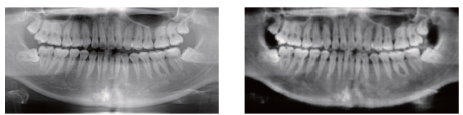
\includegraphics[width=0.45\textwidth]{nebla.png} &
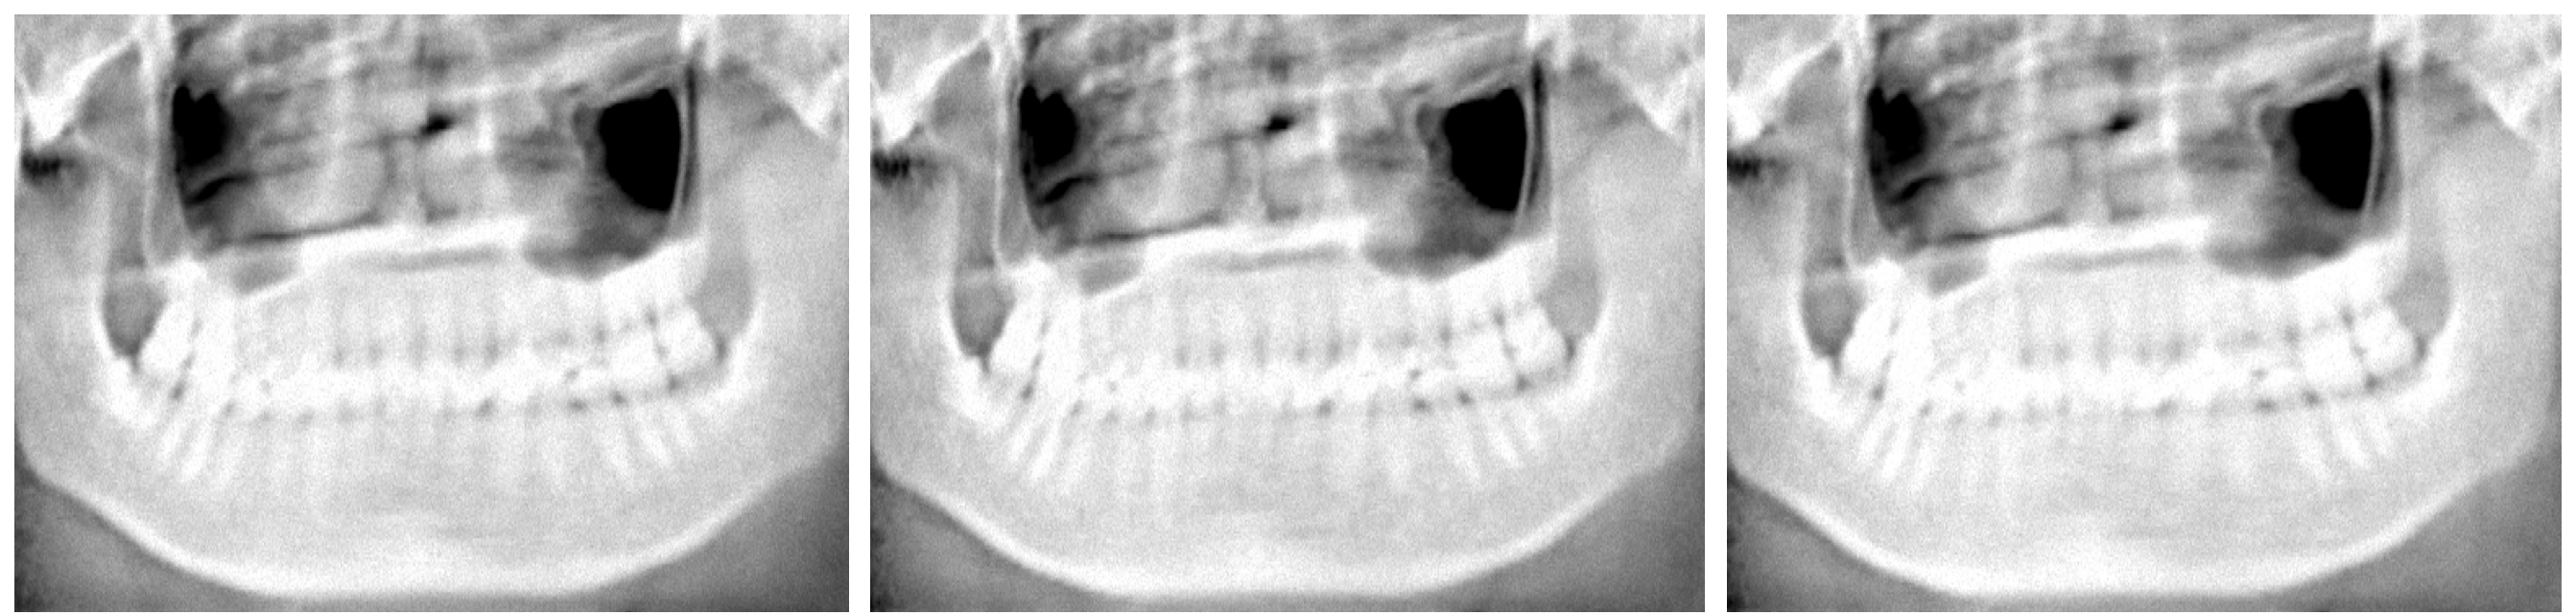
\includegraphics[width=0.45\textwidth]{rotation_comparison_minus3_0_plus3.png} \\
\small (a) NeBLa reference panoramic output & \small (b) Our generated outputs ($-3^\circ$, $0^\circ$, $+3^\circ$)
\end{tabular}
\caption{Visual comparison between (a) the NeBLa reference panoramic output style (used as contextual benchmark) and (b) the multi-view panoramic DRRs generated by our curved-arch Beer-Lambert pipeline at three rotation augmentation settings. Both show characteristic panoramic dental anatomy, validating the realism of our synthetic generation approach.}
\label{fig:nebla_vs_ours}
\end{figure*}

% =========================================================
\section{Discussion}
\label{sec:discussion}
% =========================================================

\subsection{Analysis of Results}

The pipeline achieves stable synthetic panoramic generation across all 21 CBCT volumes. The cross-view self-consistency scores (L1\,=\,0.02687, SSIM\,=\,0.7467, PSNR\,=\,29.70\,dB for the identity condition under the dynamic arch) are in the same range as values reported in the dental 2D-to-3D literature; NeBLa, for instance, reports PSNR of 19.89--21.68\,dB and SSIM of 79.21--82.62\% for the harder problem of full 3D reconstruction \cite{park2024nebla}. The dynamic, patient-adaptive curved arch substantially improves anatomical relevance compared with a naive planar parallel projection or a single hard-coded arch shared across all subjects, since the tooth crowns and roots are maintained within the focal band throughout the panoramic sweep across patients with different jaw sizes---an observation also reported for patient-tailored simulated geometry approaches \cite{sunilkumar2025panoramic} and adaptive elliptical projection paths \cite{parida2025vit}.

The pixel quality statistics (mean 0.702, std 0.217, dark fraction 2.7\%, bright fraction 16.6\%) fall within clinically reasonable ranges for panoramic radiography, and all 21 images passed automated quality checks. Average generation time of 2.23\,s per volume on CPU makes the pipeline practical for batch dataset construction without GPU requirements.

\subsection{Limitations}

Several limitations are acknowledged, consistent with known challenges in dental 2D--3D reconstruction \cite{park2024nebla,parida2025vit,wang2024neural,shin2025sparse} and CBCT synthesis \cite{sunilkumar2024recent,sunilkumar2025panoramic}:

\begin{itemize}
    \item \textbf{Heuristic attenuation calibration:} the HU-to-attenuation mapping uses fixed tissue-class thresholds rather than scanner-specific physical calibration. Scanner variability across CBCT machines may require adaptation of these parameters \cite{oliveira2025digital}.
    \item \textbf{Bone-mask-driven arch estimation:} although the arch is now dynamic and patient-adaptive, the detector still relies on a bone-attenuation threshold and morphological operations. Patients with severe bone loss, large metallic artefacts, or atypical arch morphology may require threshold adjustment or more robust estimators in the spirit of \cite{abdi2015automatic,lian2020deep}.
    \item \textbf{Fixed focal-trough and post-processing parameters:} the 30\,mm focal-trough depth and post-processing parameters are fixed across all volumes. Patient-specific calibration of these parameters may further improve image fidelity.
    \item \textbf{Downsampled volume resolution:} resampling to $128^3$ reduces fine anatomical detail. Future work may explore higher-resolution projections at the cost of increased computation.
    \item \textbf{Absence of soft-tissue reconstruction:} the current pipeline projects bone and soft tissue through a unified attenuation map but does not separately reconstruct soft tissues, nerves, or periodontal structures.
\end{itemize}

% =========================================================
\section{Conclusion and Future Work}
\label{sec:conclusion}
% =========================================================

This paper presents and evaluates a complete, physics-grounded pipeline for generating synthetic panoramic dental X-rays from CBCT volumes. The pipeline implements Beer--Lambert attenuation physics through a curved-focal-trough ray-tracing formulation, dynamically auto-fits a patient-adaptive parabolic dental arch geometry per volume from a CLAHE-enhanced bone-density projection, and produces multi-view augmented paired training data suitable for downstream 2D-to-3D dental reconstruction models.

Applied to 21 CBCT scans, the pipeline generated 63 augmented panoramic--CBCT pairs with cross-view quality metrics of L1\,=\,0.02687, SSIM\,=\,0.7467, and PSNR\,=\,29.70\,dB (identity condition under the dynamic arch), and exported a 187.2\,MB PyTorch-format paired dataset. All quality verification checks passed across the full dataset.

Future directions include:
\begin{itemize}
    \item \textbf{Machine-specific trajectory modelling:} developing methods to automatically estimate patient- and scanner-specific X-ray acquisition trajectories for improved DRR realism \cite{park2024nebla,parida2025vit,sunilkumar2025panoramic}.
    \item \textbf{Scanner-calibrated attenuation mapping:} replacing heuristic HU thresholds with scanner-specific physical calibration for more accurate radiographic simulation \cite{oliveira2025digital}.
    \item \textbf{Multi-structure reconstruction and labelling:} extending the pipeline to separately reconstruct and label teeth, jawbone, mandibular canal, and soft-tissue structures, leveraging anatomical-segmentation work such as \cite{abdi2015automatic,lian2020deep,wang2024neural}.
    \item \textbf{Higher-resolution and time-resolved DRR generation:} exploring $256^3$ or full-resolution projections, and incorporating intra-scan motion modelling along the lines of \cite{xie2025time,ramesh2024machine}.
    \item \textbf{Sparse-view reconstruction with synthetic data:} using the generated dataset to train sparse-view CBCT reconstructors such as \cite{lin2023learning,lin2024c,lin2026deepsparse,liu2024geometry,momeni2024differentiable,yang2025trans,zhang2023novel,shin2025sparse}.
    \item \textbf{Integration with single-view reconstruction pipelines:} using the paired dataset to train and evaluate 3D reconstruction models such as Oral-3D \cite{song2021oral}, Oral-3Dv2 \cite{song2023oral}, X2Teeth \cite{liang2020x2teeth}, OralViewer \cite{liang2021oralviewer}, NeBLa \cite{park2024nebla}, ViT--NeBLa \cite{parida2025vit}, PX2Tooth \cite{ma2024px2tooth}, DTR-Net \cite{mei2023dtr}, 3DPX \cite{li20243dpx}, the multi-view EfficientNetB0 model of \cite{mohamed20253d}, the impacted-canine generative model of \cite{minhas2024artificial}, and bone-surface methods such as 3DDX \cite{gu20243ddx} and the encoder--decoder benchmark of \cite{shakya2023benchmarking}.
    \item \textbf{Clinical validation:} validating the synthetic panoramics against real clinical OPG images in terms of diagnostic utility for caries detection, bone-level assessment, and implant planning.
\end{itemize}

\section*{Acknowledgment}
The authors thank the Department of Computer Science and Engineering, Sardar Vallabhbhai National Institute of Technology (SVNIT), Surat, for providing computational resources and institutional support. This work was carried out under the M.Tech. Data Science program (2024--26) at SVNIT Surat.

\bibliographystyle{IEEEtran}
\bibliography{reference}

\end{document}